
\chapter{Integración}

En este capítulo vamos a estudiar el concepto que, junto con el de derivada, forma el núcleo del cálculo diferencial e integral.
Veremos que dicho concepto, el de \emph{integral}, será definido por motivos totalmente ajenos a los que nos llevaron a definir la derivada, pero también veremos que está íntimamente conectado a través del teorema fundamental del cálculo.

\section{La integral definida de una función continua}
% Seguimos el Salas-Hille

La noción de integral definida como la presentaremos aquí aparece naturalmente cuando se intenta resolver el problema del cálculo del área de una región plana. El lector recordará la fórmula del área de ciertas figuras planas, por ejemplo el rectángulo el triángulo, el círculo, etc.

\centerline{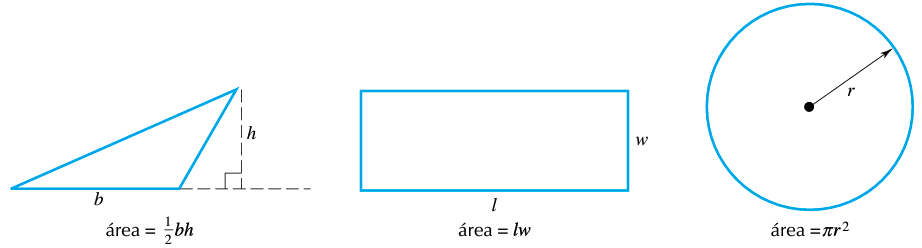
\includegraphics[width=.8\textwidth]{pics/areas-simples.png}}

En este capítulo veremos cómo calcular el área de figuras más generales. Comenzaremos con el cálculo del área que queda delimitada de la siguiente manera:

\noindent
\begin{minipage}{.5\textwidth}
  \begin{itemize}
  \item Por debajo, por el eje $x$;
  \item Por encima, por la gráfica de $y=f(x)$;
  \item A la izquierda por la recta $x=a$; 
  \item A la derecha por la recta $x=b$.
\end{itemize}
\end{minipage}
\begin{minipage}{.5\textwidth}
  \centering
  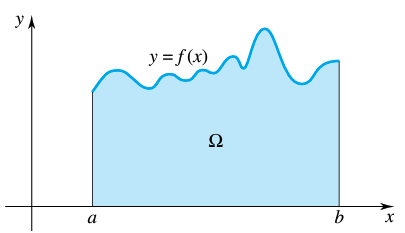
\includegraphics[width=.9\textwidth]{pics/area-bajo-curva.png}
\end{minipage}

\noindent
\begin{minipage}{.5\textwidth}
  Consideramos ahora una subdivisión del intervalo $[a,b]$ en un número finito de subintervalos que no se solapan:
  \[
  [x_0,x_1],\ [x_1,x_2],\dots,\ [x_{n-1},x_n]
  \]
  con $\D a=x_0<x_1<\dots<x_n=b$.

  Observamos que el área de la región $\Omega$ es lo mismo que la suma de las áreas de las regiones $\Omega_i$.
\end{minipage}
\begin{minipage}{.5\textwidth}
  \centering
  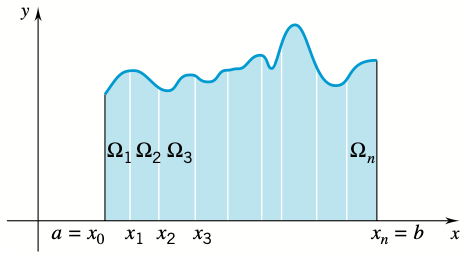
\includegraphics[width=.9\textwidth]{pics/area-bajo-curva-particionada.png}
\end{minipage}

Podemos aproximar el área total de $\Omega$ aproximando el área de cada una de las subregiones $\Omega_i$ y sumando los resultados.
Definimos, para cada $i=1,2,\dots,n$ las siguientes cantidades:
\[ 
  m_i = \min_{x\in [x_{i-1},x_i]}f(x)=\min_{[x_{i-1},x_i]}f,
  \qquad
  M_i = \max_{x\in [x_{i-1},x_i]}f(x)=\max_{[x_{i-1},x_i]}f.
\]
Luego, si $r_i = [x_{i-1},x_i]\times [0,m_i]$ y $R_i = [x_{i-1},x_i]\times [0,M_i]$, resulta que
\[
r_i \subset \Omega_i \subset R_i
\quad\text{y entonces}\quad
\area(r_i)\le \area(\Omega_i) \le \area(R_i).
\]

\centerline{
  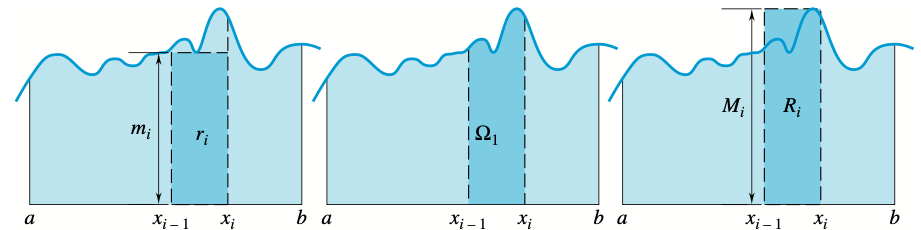
\includegraphics[width=.9\textwidth]{pics/area-omega-i.png}
}

Dado que el área de un rectángulo es el producto de la base por la altura, obtenemos
\[
m_i\, (x_i-x_i-1)
\le \area(\Omega_i) \le
M_i\, (x_i-x_i-1),
\qquad\text{para $i=1,2,\dots,n$}.
\]
Definiendo $\Delta x_i=x_i-x_{i-1}$ tenemos que 
\[
m_i\, \Delta x_i
\le \area(\Omega_i) \le
M_i\, \Delta x_i,
\qquad\text{para $i=1,2,\dots,n$}.
\]
Sumando, obtenemos
\begin{equation}
  \label{eq:L<I<U}
m_1 \Delta x_1 + m_2 \Delta x_2 + \dots + m_n \Delta x_N
\le \area(\Omega_i) \le
M_1 \Delta x_1 + M_2 \Delta x_2 + \dots + M_n \Delta x_N.
\end{equation}
La suma $m_1 \Delta x_1 + m_2 \Delta x_2 + \dots + m_n \Delta x_N$ es una \emph{suma inferior de $f$} 
y la suma $M_1 \Delta x_1 + M_2 \Delta x_2 + \dots + M_n \Delta x_N$ es una \emph{suma superior de $f$}.

\centerline{
  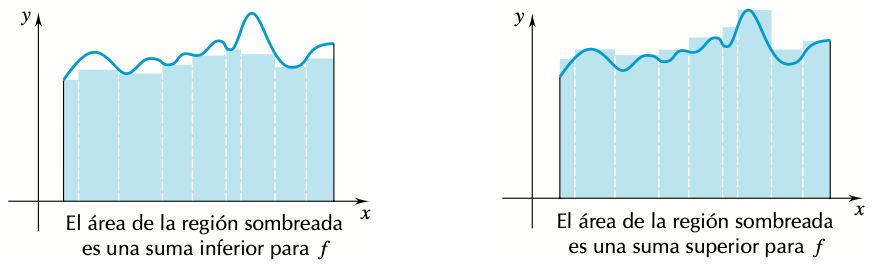
\includegraphics[width=.9\textwidth]{pics/sumas-superiores-inferiores.png}
}

La desigualdad~\eqref{eq:L<I<U} nos dice que para que un número pueda ser candidato al título de \emph{área de $\Omega$}, tal número ha de ser mayor o igual que cualquier suma inferior de $f$ y menor o igual que cualquier suma superior de $f$. Puede demostrarse, aunque no lo veremos aquí, que si $f$ es una función continua en $[a,b]$ entonces existe un número y sólo uno que cumple estas condiciones. A tal número lo llamaremos \emph{área de $\Omega$}.

\subsection*{Integral definida}

El procedimiento seguido para resolver el problema de área se llama \emph{integración} y el resultado final de este procedimiento se denomina \emph{integral definida}. A continuación estableceremos estas nociones con más precisión.

\begin{definition}
  Llamaremos \emph{partición} del intervalo cerrado $[a,b]$ a todo subconjunto finito de $[a,b]$ que contenga a los extremos. Es conveniente identificar los elementos de la partición con un índice acorde al orden narural. Así, cuando escribimos que 
  \[
  P=\{x_0,x_1, \dots ,x_n\} \text{ es una partición de $[a,b]$},
  \]
  entendemos que $\D a=x_0<x_1<\dots<x_n=b$.
\end{definition}

Supongamos ahora que $f$ es una función continua sobre $[a,b]$. En cada subintervalo $[x_{i-1},x_i]$ la función $f$ toma entonces un valor máximo $M_i$ y un mínimo $m_i$. Definimos entonces:

\begin{definition}
  Sea $f$ una función continua sobre $[a,b]$ y sea $P=\{a=x_0<x_1<\dots<x_n=b\}$ una partición de $[a,b]$. Luego definimos, para cada $i=1,2,\dots,n$:
  \[ 
    m_i = \min_{[x_{i-1},x_i]}f,
    \qquad
    M_i = \max_{[x_{i-1},x_i]}f.
  \]
  El número 
  \[
  L(P,f)= m_1 \Delta x_1 + m_2 \Delta x_2 + \dots + m_n \Delta x_N 
  = \sum_{i=1}^n m_i \Delta x_i,
  \]
  se denomina
  \emph{suma inferior de $f$ correspondiente a la partición $P$};
  y el número 
  \[
  U(P,f)= M_1 \Delta x_1 + M_2 \Delta x_2 + \dots + M_n \Delta x_N
  = \sum_{i=1}^n M_i \Delta x_i,
  \]
  se denomina \emph{suma superior de $f$ correspondiente a la partición $P$}.
\end{definition}

\begin{theorem}
  Si $f$ es una función continua en $[a,b]$ existe un único número $I$ que satisface la desigualdad 
  \[
  L(P,f)\le I\le U(P,f),
  \qquad\text{para toda partición $P$ de $[a,b]$}
  \]
\end{theorem}

\begin{proof}
  La demostración de este teorema queda fuera del alcance de este apunte, y será discutida en las clases de Coloquio de Demostraciones.
\end{proof}

A partir de este último teorema llegamos a la definición principal de esta sección:

\begin{definition}[Integral definida]
  Sea $f$ una función continua en $[a,b]$. El único número $I$ que satisface 
  \[
    L(P,f)\le I\le U(P,f),
    \qquad\text{para toda partición $P$ de $[a,b]$}
  \]
  se llama \emph{integral definida} (o simplemente \emph{integral}) de $f$ entre $a$ y $b$ y se designa por
  \[
  \int_a^b f(x)\dx.
  \]
\end{definition}

El símbolo $\int$ fue introducido por Leibniz y se llama \emph{signo integral}. En realidad es una \emph{S} (de \emph{suma}) estirada. Los números $a$ y $b$ se denominan \emph{límites de integración} ($a$ es el límite inferior y $b$ el límite superior). La función a integrar se llama \emph{integrando}. En algunos libros suele escribirse más brevemente $\int_a^b f$, omitiendo la variable $x$.

En la expresión $\int_a^b f(x)\dx$ la variable $x$ es una \emph{variable muda}. Esto quiere decir que puede ser sustituida por cualquier otra letra no utilizada hasta el momento. Así:
\[
\int_a^b f(x)\, dx
= \int_a^b f(t)\, dt
= \int_a^b f(u)\, du
= \int_a^b f(z)\, dz.
\]

En la introducción a este capítulo comenzamos con una aplicación inmediata de la integral definida:
Si $f$ es no negativa en $[a,b]$, entonces
\[
A = \int_a^b f(x)\dx
\]
da como resultado el área debajo de la gráfica de $f$.
Volveremos más adelante sobre esta aplicación.
Ahora veamos algunos ejemplos sencillos que nos ayudarán a comprender la definición.

\begin{example}
  Si $f(x)=c$, una constante, para todo $x\in[a,b]$, ?`cuánto vale $\int_a^b f(x)\dx$?

  Veamos, si $P=\{a=x_0<x_1<\dots<x_n=b\}$ es una partición de $[a,b]$, tenemos que 
\[ 
    m_i = \min_{[x_{i-1},x_i]}f = c
    \qquad
    M_i = \max_{[x_{i-1},x_i]}f = c;
  \]
  por lo que 
  \[
  L(P,f)
  = \sum_{i=1}^n m_i \Delta x_i
  = \sum_{i=1}^n c \Delta x_i
  = c \sum_{i=1}^n \Delta x_i
  = c (b-a)
  \]
  y 
  \[
  U(P,f)
  = \sum_{i=1}^n M_i \Delta x_i
  = \sum_{i=1}^n c \Delta x_i
  = c \sum_{i=1}^n \Delta x_i
  = c (b-a).
  \]
  Luego, 
  \[
    L(P,f)\le c(b-a)\le U(P,f),
    \qquad\text{para toda partición $P$ de $[a,b]$},
  \]
  y concluimos que 
  \[
  \int_a^b f(x)\dx = \int_a^b c \dx = c (b-a).
  \]

  Como ejemplos concretos:
  \begin{align*}
    \int_{-1}^1 3 \dx = 3 \big(1 - (-1)\big) = 3 \cdot 2 = 6;
    % \qquad\text{y}
    \\
    \int_{4}^{10} -3 \dx = -2 \big(10 - 4\big) = -2 \cdot 6 = -12.
  \end{align*}
\end{example}

\begin{example}
  Nos proponemos estudiar ahora la integral de la función $f(x)=x$, es decir $\int_a^b x\dx$.
  Veamos, si $P=\{a=x_0<x_1<\dots<x_n=b\}$ es una partición de $[a,b]$, tenemos que 
  \[ 
      m_i = \min_{[x_{i-1},x_i]}f = x_{i-1}
      \qquad
      M_i = \max_{[x_{i-1},x_i]}f = x_i;
    \]
    por lo que 
    \[
    L(P,f)
    = \sum_{i=1}^n m_i \Delta x_i
    = \sum_{i=1}^n x_{i-1} (x_{i}-x_{i-1})
    \]
    y 
    \[
    U(P,f)
    = \sum_{i=1}^n M_i \Delta x_i
    = \sum_{i=1}^n x_{i} (x_{i}-x_{i-1}).
    \]
    Observamos que para cada índice $i=1,2,\dots,n$, 
    \[
    x_{i-1}\le \frac12 (x_i+x_{i-1})\le x_i.
    \]
    Luego, multiplicando por $\Delta x_i = x_i-x_{i-1}>0$, tenemos que
    \[
    x_{i-1} \Delta x_i 
    \le \frac12 (x_i+x_{i-1})(x_i-x_{i-1}) 
    = \frac12 (x_i^2-x_{i-1}^2) = 
    \le x_i \Delta x_i.
    \]
    Sumando para $i$ de $1$ a $n$ obtenemos
    \[
    L(P,f) \le \sum_{i=1}^n \frac12 (x_i^2-x_{i-1}^2) \le U(P,f).
    \]
    Pero 
    \begin{align*}
      \sum_{i=1}^n \frac12 (x_i^2-x_{i-1}^2)
      &= \frac12 \Big[ (x_1^2-x_0^2) + (x_2^2-x_1^2) + \dots + (x_n^2-x_{n-1}^2)  \Big]
      \\
      &= \frac12 \big(x_n^2-x_0^2\big)
      = \frac12 \big(b^2-a^2\big).
    \end{align*}
    Luego, 
    \[
      L(P,f)\le \frac12 \big(b^2-a^2\big) \le U(P,f),
      \qquad\text{para toda partición $P$ de $[a,b]$},
    \]
    y por lo tanto
    \[
    \int_a^b x\dx = \frac12 \big(b^2-a^2\big).
    \]
    Como ejemplos concretos:
    \begin{align*}
      \int_{-1}^1 x \dx = \frac12 \big(3^2 - (-1)^2\big) = \frac12 \cdot 8 = 4;
      % \qquad\text{y}
      \\
      \int_{-2}^{2} x \dx = \frac12 \big(2^2 - (-2)^2\big) = \frac12 \cdot 0 = 0.
    \end{align*}\end{example}

\begin{example}
  Consideremos un último ejemplo, de una función \emph{discontinua}, pero \emph{continua a trozos}.
  Sea 
  \[
  f(x)=\begin{cases}
    0, \quad&\text{si $x\neq 1$},
    \\
    1, \quad&\text{si $x=1$}.
  \end{cases}
  \]
  Afirmamos que $\int_0^2 f(x)\dx=0$, es decir, cambiar el valor de la función en un punto no afecta el valor de la integral.
  Claramente, cualquiera sea la partición $P$ del intervalo $[0,2]$, se tiene que 
  \[
  0=L(P,f) \le 0 \le U(P,f).
  \]
  Veamos que $0$ es el único número que cumple dicha desigualdad para toda partición.
  Consideremos la partición $P_\epsilon = \{0, 1-\epsilon, 1+\epsilon, 2\}$, para $0<\epsilon<1$.
  Luego, $L(P_\epsilon,f)=0$ y 
  \[
  U(P,f)=0 (x_1-x_0) + 1 (x_2-x_1) + 0 (x_3-x_2)
  = (x_2-x_1)= \big((1+\epsilon)-(1-\epsilon)\big)=2\epsilon.
  \]
  El único número que cumple $0\le I \le 2\epsilon$ para todo $\epsilon\in(0,1)$ es $I=0$.
  Por lo tanto $\int_0^2 f(x)\dx=0$.
\end{example}


\subsubsection*{Ejercicios de la sección~\getcurrentref{chapter}.\getcurrentref{section}}

\begin{enumerate}
\item Hallar $L(P,f)$ y $U(P,f)$ en cada uno de los siguientes casos:
\begin{enumerate}
  \item $\D f(x) = 1-x$, $P=\{0, \frac13, \frac34, 1, 2\}$
  \item $\D f(x) = \sqrt{x}$, $P=\{0, \frac1{25}, \frac4{25}, \frac9{25}, \frac{16}{25}, 1\}$
  \item $\D f(x) = x^2$, $P=\{-1,-\frac12, -\frac14, 0, \frac14, \frac12, 1\}$
\end{enumerate}

\item Sea $f$ una función continua en $[-1,1]$. Explicar por qué cada una de las siguientes afirmaciones es falsa.
\begin{enumerate}
  \item $L(P,f)=3$ y $U(P,f)=2$.
  \item $L(P,f)=3$ y $U(P,f)=6$ y $\int_{-1}^1 f(x)\dx=2$.
  \item $L(P,f)=3$ y $U(P,f)=6$ y $\int_{-1}^1 f(x)\dx=10$.
\end{enumerate}

\item Sea $f:[0,1]\to \R$ definida por
\[
\begin{cases}
  1, \quad&\text{si $x\in\Q$,}
 \\ 
 0, \quad&\text{si $x\notin\Q$.}
\end{cases}
\]
Si $P$ es una partición de $[0,1]$.
?`Cuánto valen $L(P,f)$ y $U(P,f)$?
?`Cuántos números $I$ hay que cumplen $L(P,f) \le I \le U(P,f)$, para toda partición $P$?
\end{enumerate}


\section{El Teorema Fundamental del Cálculo}
  %La función \texorpdfstring{$F(x)=\int_a^x f(t)\dx$}{integral hasta \emph{x}}}

En los ejemplos de la sección anterior tuvimos que confiar en que se nos ocurriera una idea para saber cómo encontrar el número $I$ que da la integral. En esta sección estudiaremos propiedades de la integral que nos permitirán encontrar una forma más sistemática y sencilla de calcular integrales.

Para ello necesitamos primero la siguiente Proposición.

\begin{proposition}
  Sea $f$ es continua en $[a,b]$, y sean $P$ y $Q$ dos particiones del intervalo $[a,b]$.
  Si $P\subset Q$, entonces 
  \[
  L(P,f) \le L(Q,f)
  \qquad\text{y}\qquad
  U(Q,f) \le U(P,f).
  \]
  Es decir, al agregar puntos a una partición, \emph{las sumas inferiores crecen} y \emph{las sumas superiores decrecen}.
\end{proposition}

\begin{proof}
  Basta con probar el caso en que $Q$ tiene un punto más que $P$, luego proceder por inducción.
  Supongamos entonces que $P=\{a=x_0<x_2<\dots<x_n=b\}$ y que $Q = P\cup \{p\}$. Sea $i_0\in\{x_1,x_2,\dots,x_n\}$ tal que $x_{i_0-1}<p<x_{i_0}$.
  Gráficamente, la situación en ese intervalo se vería así:

  \centerline{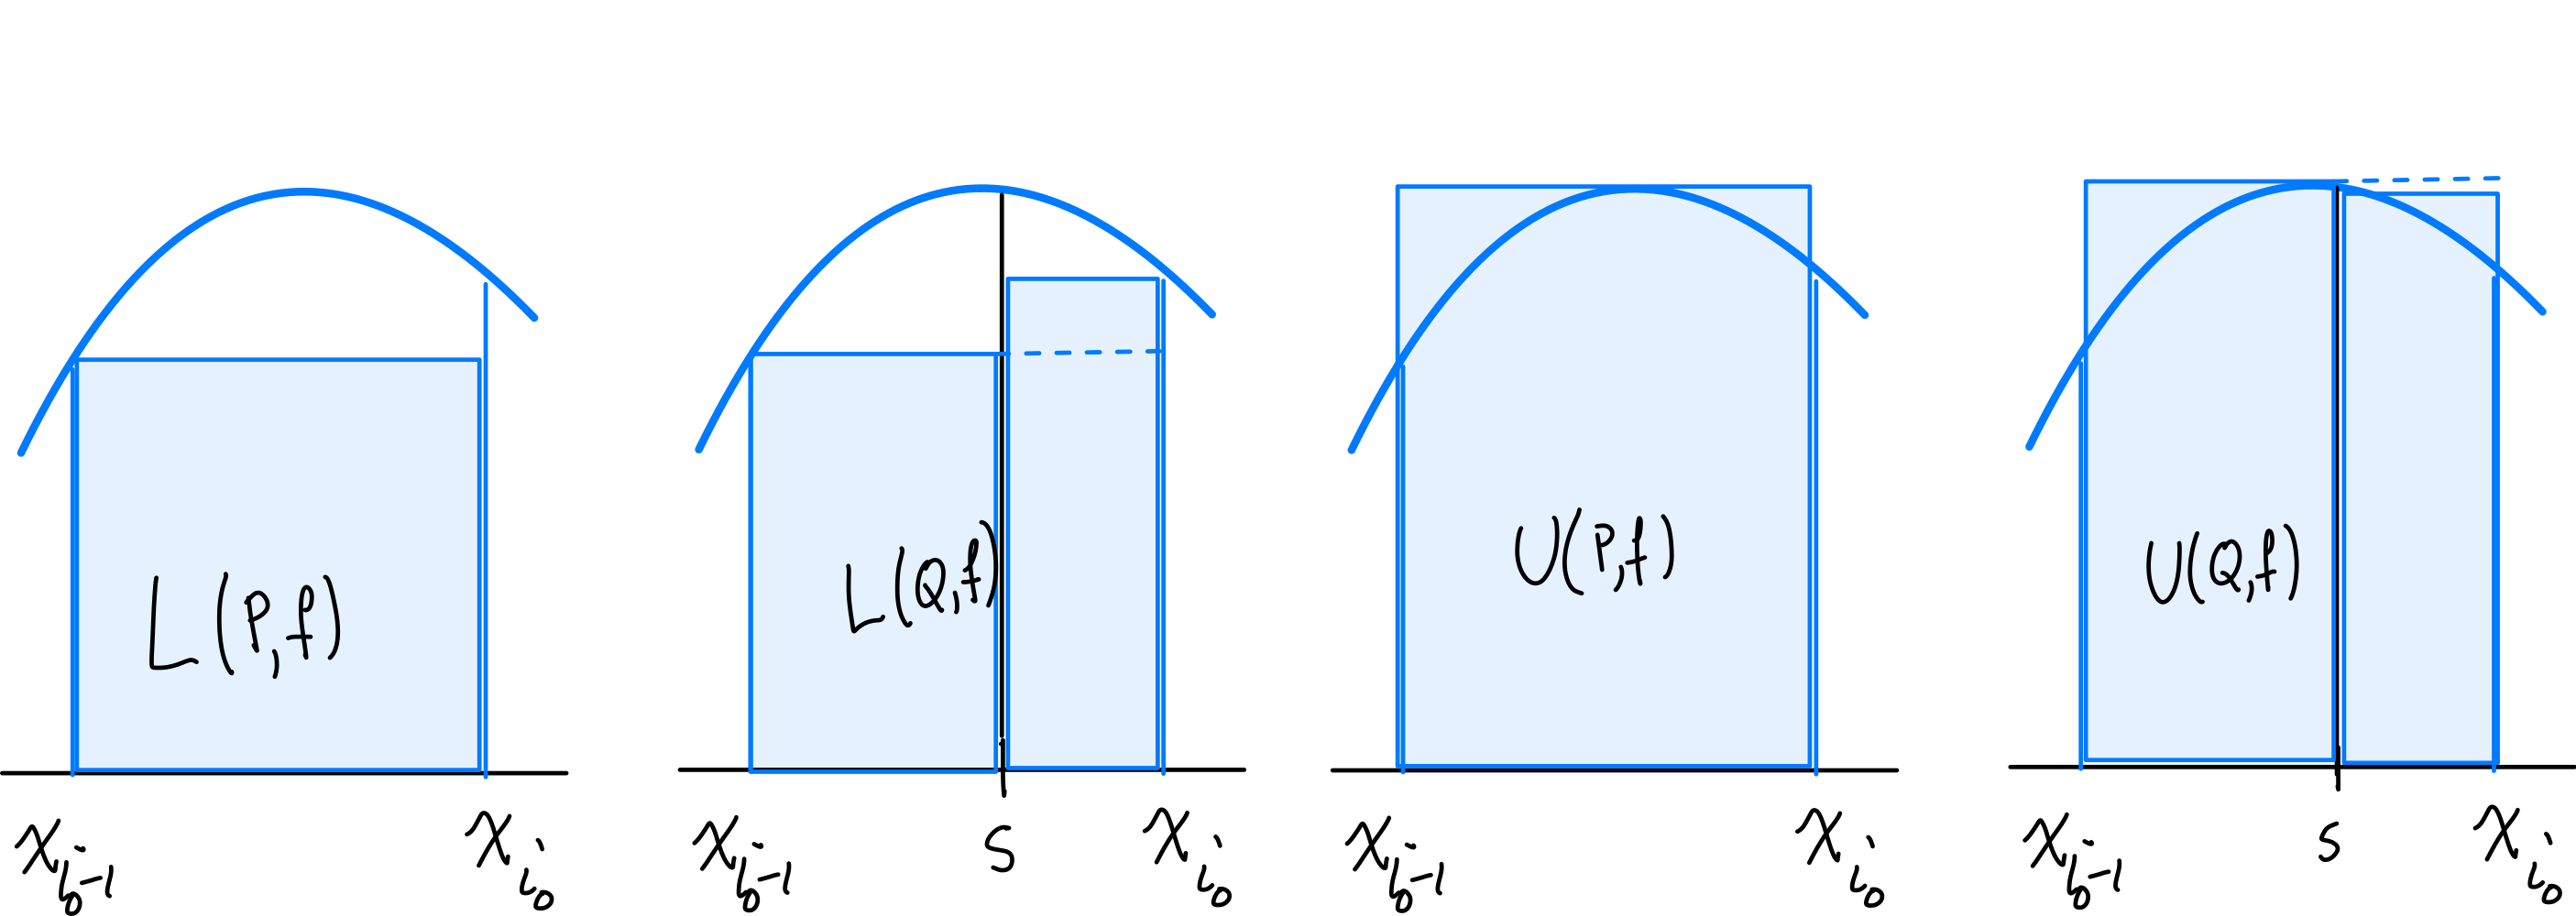
\includegraphics[width=.8\textwidth]{pics/sumas-insertar-punto.png}}

  Por lo tanto, el único término de la suma inferior de $P$ que se cambia, cambia por dos términos que al sumarlos dan mayor o igual al término original.
  Y el único término de la suma superior de $P$ que se cambia, cambia por dos términos que al sumarlos dan menor o igual al término original. 
  De aquí concluimos la afirmación de la proposición.
\end{proof}

El siguiente teorema es bastante obvio si pensamos en la interpretación geométrica de la integral como un área.

\begin{theorem}
  Si $f$ es continua en $[a,b]$ y $a<c<b$, entonces
  \[
  \int_a^b f(x)\dx = \int_a^c f(x)\dx + \int_c^b f(x)\dx.
  \]
\end{theorem}

\noindent
\begin{minipage}{.6\textwidth}
  \[ \area(I)+\area(II)=\area(\text{región completa})\]
\end{minipage}
\begin{minipage}{.39\textwidth}
\centerline{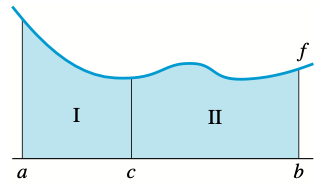
\includegraphics[width=.8\textwidth]{pics/integral-suma-intervalos.png}}
\end{minipage}

\begin{proof}
  Para demostrar el teorema basta con que demostremos que para toda partición $P$ de $[a,b]$ se verifica que
  \[
  L(P,f) \le \int_a^c f(x)\dx + \int_c^b f(x)\dx \le U(P,f).
  \]
  Consideremos entonces una partición arbitraria $P$ de $[a,b]$ y sea $Q=P\cup\{c\}\supset P$.
  Por la proposición anterior 
  \[
  L(P,f) \le L(Q,f)
  \qquad\text{y}\qquad
  U(Q,f) \le U(P,f).
  \]
  Ahora consideramos subparticiones de $Q$ en los intervalos $[a,c]$ y $[c,b]$:
  \[
  Q_1 = Q\cap[a,c]\qquad\text y\qquad 
  Q_2 = Q\cap[c,b].
  \]
  Luego $Q_1$ y $Q_2$ son particiones de $[a,c]$ y de $[c,b]$ respectivamente, por lo tanto:
  \[
  L(Q_1,f)\le \int_a^c f(x)\dx \le U(Q_1,f)
  \qquad\text{y}\qquad
  L(Q_2,f)\le \int_c^b f(x)\dx \le U(Q_2,f).
  \]
  Sumando estas desigualdades obtenemos
  \[
  L(Q_1,f)+L(Q_2,f)\le \int_a^c f(x)\dx + \int_c^b f(x)\dx \le U(Q_1,f)+U(Q_2,f).
  \]
  Finalmente observamos que 
  \[
    L(Q_1,f)+L(Q_2,f) = L(Q,f)
    \qquad\text y\qquad
    U(Q_1,f)+U(Q_2,f) = U(Q,f),
  \]
  que implica lo que queríamos demostrar.
  \end{proof}

  Hasta ahora sólo hemos definido integrales \emph{de izquierda a derecha}: desde un número $a$ hasta un número $b$, con $b>a$. También puede integrarse en sentido opuesto, a través de la siguiente definición:
  \[
  \int_b^a f(x)\dx 
  = -\int_a^b f(x)\dx .
  \]
  Además, la integral cuando los extremos de integración coinciden se define como cero:
  \[
  \int_c^c f(x)\dx = 0.
  \]
  De esta manera, la siguiente condición se cumple independientemente del orden en que se encuentren $a$, $b$ y $c$:
  \[
    \int_a^c f(x)\dx + \int_c^b f(x)\dx=\int_a^b f(x)\dx .
  \]

\noindent
\begin{minipage}{.4\textwidth}  Dada una función continua $f$, definimos 
  \[
  F(x)=\int_a^x f(t)\dt.
  \]
  Es decir, $F(x)$ es el área de la región sombreada en las figuras, que varía al variar $x$.
\end{minipage}
\begin{minipage}{.6\textwidth}
  \begin{center}
    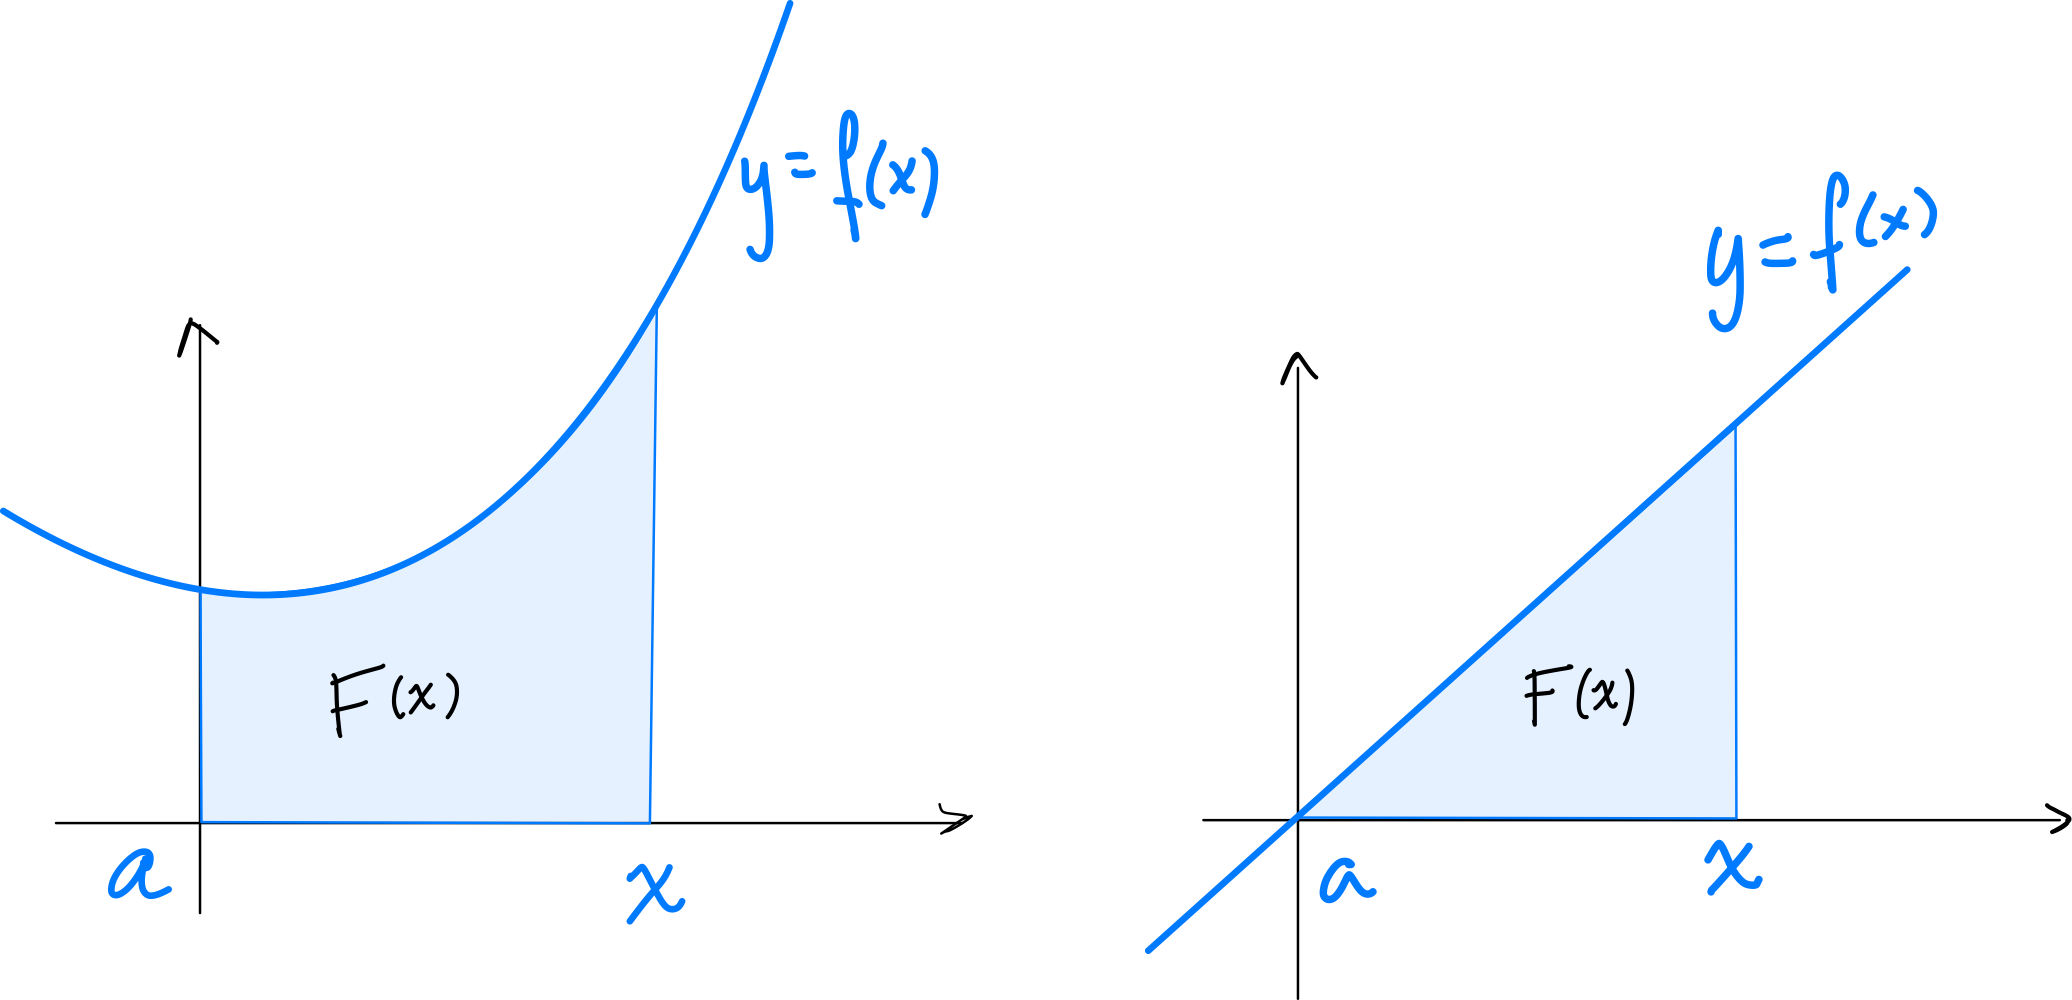
\includegraphics[width=.95\textwidth]{pics/integral-hasta-x.png}
  \end{center}
\end{minipage}

El siguiente teorema se conoce como Teorema Fundamental del Cálculo, y relaciona el concepto nuevo de integral con el de derivada, de la siguiente manera:

\begin{theorem}\label{T:TFC}
  Si $f$ es continua en $[a,b]$ y definimos $F:[a,b]\to\R$ como 
  \[
  F(x)=\int_a^x f(t)\dt,
  \]
  Entonces $F$ es continua en $[a,b]$ y diferenciable en $(a,b)$ y más aún, 
  \[
  F'(x)=f(x),\quad\text{para todo $x\in(a,b)$.}
  \]
\end{theorem}

\begin{proof}
  Comenzamos considerando $x\in[a,b)$ y veremos que 
  \[\lim_{h\to 0^+}\frac{F(x+h)-F(x)}{h}=f(x).\]
  Si $x<x+h\le b$, entonces
  \[F(x+h)-F(x)=\int_a^{x+h}f(t)\dt - \int_a^x f(t)\dt = \int_x^{x+h}f(t)\dt.\]
  Definimos ahora 
  $$ M_h = \max_{[x,x+h]}f\qquad\text y\qquad
  m_h = \min_{[x,x+h]}f.$$
  Entonces, 
  $$ M_h \cdot \big( (x+h)-x \big) = M_h \cdot h $$
  es una suma superior para $f$ en $[x,x+h]$ y
  $$ m_h \cdot \big( (x+h)-x \big) = m_h \cdot h $$ 
  es una suma inferior para $f$ en $[x,x+h]$.
  Luego
  $$ m_h \cdot h \le \int_x^{x+h}f(t)\dt \le M_h\cdot h,$$
  que a su vez implica
  $$ m_h \le \frac{\int_x^{x+h}f(t)\dt}h \le M_h.$$
  Es decir,
  $$ m_h \le \frac{F(x+h)-F(x)}h \le M_h.$$
  Como $f$ es continua en $[a,b]$
  \[
  \lim_{h\to0^+} m_h = f(x) = \lim_{h\to 0^+} M_h,
  \]
  y por el teorema del emparedado
  \begin{equation}\label{eq:TFC-der}
    \lim_{h\to 0^+} \frac{F(x+h)-F(x)}h = f(x).
  \end{equation}

  De manera análoga se puede demostrar que, para $x\in(a,b]$ se verifica
  \begin{equation}\label{eq:TFC-izq}
    \lim_{h\to 0^-} \frac{F(x+h)-F(x)}h = f(x).
  \end{equation}
  Esto implica que para $x\in(a,b)$ se cumplen~\eqref{eq:TFC-der} y~\eqref{eq:TFC-der} a la vez, 
  \[
  F'(x)= \lim_{h\to 0} \frac{F(x+h)-F(x)}h = f(x).
  \]
  Esto muestra que $F(x)$ es diferenciable en $(a,b)$ y su derivada es $F'(x)=f(x)$.

  Solo queda probar que $F$ es continua por derecha en $a$ y continua por izquierda en $b$.
  A partir de~\eqref{eq:TFC-der} en $a$ obtenemos
  $$ 
  \lim_{h\to 0^+} \frac{F(a+h)-F(a)}h = f(a),
  $$ 
  Que a su vez implica que
  $$ 
  \lim_{h\to 0^+} \big(F(a+h)-F(a)\big)
  = \lim_{h\to 0^+}\Big( h\cdot \frac{F(a+h)-F(a)}h \Big)= f(a)\cdot 0 = 0.
  $$ 
  Por lo tanto $\lim_{h\to 0^+} F(a+h)=F(a)$ y $F$ es continua por derecha en $a$.
  Análogamente se puede demostrar que $F$ es continua por izquierda en $b$, usando~\eqref{eq:TFC-izq}.
\end{proof}

\begin{example}
  Si $F$ está definida por 
  \[
  F(x)=\int_{-1}^x (2t+t^2) \dt,
  \qquad \text{para $-1\le x\le 5$},
  \]
  Entonces $F'(x) = 2x+x^2$.
\end{example}


\begin{example}
  Si $F$ está definida por 
  \[
  F(x)=\int_{0}^x \sen(\pi t) \dt,
  \qquad \text{para $x\in\R$},
  \]
  Entonces $F'(x) = \sen(\pi x)$.
\end{example}

A continuación veremos cómo este teorema nos sirve para calcular integrales definidas de un gran número de funciones. Para ello hacemos primero la siguiente definición.

\begin{definition}[Antiderivada]
  Sea $f$ una función continua en $[a,b]$. Una función $G$ se llama \emph{antiderivada} de $f$ en $[a,b]$ si y sólo si
  \[
  G\text{ es continua en $[a,b]$ \quad y \quad}
  G'(x)=f(x) \text{ para todo $x\in(a,b)$.}\]
\end{definition}

El Teorema~\ref{T:TFC} nos dice que, si $f$ es continua en $[a,b]$, entonces la función $F(x)$ definida por 
\[
  F(x)=\int_a^x f(t)\dt.
\]
es una antiderivada de $f$.
A partir del \emph{Teorema Fundamental del Cálculo} llegamos a un método que nos permite calcular integrales. Podemos calcular $\D\int_a^b f(t)\dt$ hallando una antiderivada de $f$.

\begin{theorem}[Regla de Barrow]
   Sea $f$ una función continua en $[a,b]$. Si $G$ es una antiderivada de $f$ en $[a,b]$, entonces
   $$ \int_a^b f(t)\dt = G(b)-G(a). $$
\end{theorem}

\begin{proof}
  Consideremos la función $F:[a,b]\to \R$ definida por $\D  F(x)=\int_a^x f(t)\dt$. 
  Luego, por un lado, 
  $$F(a)=\int_a^a f(t)\dt = 0,\qquad\text y\qquad  F(b)=\int_a^b f(t)\dt.$$

  Por otro lado, por el Teorema~\ref{T:TFC},
  $F(x)$ es una antiderivada de $f$, al igual que $G$. Luego,
  \[
  F'(x)=f(x)\quad\text y\quad G'(x)=f(x),\qquad\text{para todo $x\in(a,b)$.}
  \]
  Por el Corolario~\ref{C:f=g+k}, resulta que existe una constante $k\in\R$ tal que 
  \[
  F(x) = G(x) + k,
  \qquad\text{para todo $x\in[a,b]$.}
  \]
  Como $F(a)=0$, resulta que $G(a)+k=0$, es decir, $k = -G(a)$.
  Por lo tanto
  \[
  F(x) = G(x) - G(a),
  \qquad\text{para todo $x\in[a,b]$.}
  \]
  En particular, 
  \[
  F(b) = \int_a^b f(t)\dt = G(b)-G(a),
  \]
  que es lo que se quería demostrar.
\end{proof}

De este último teorema, obtenemos un procedimiento para calcular integrales.
\begin{quote}
  Para calcular $\D\int_a^b f(t)\dt$, debemos hacer lo siguiente:
  \begin{enumerate}
    \item Hallar una antiderivada $G$ de $f$.
    \item Calcular $G(b)-G(a)$. Ese resultado es $\D\int_a^b f(t)\dt$.
    \item FIN.
  \end{enumerate}
\end{quote}


\begin{example}
  Calcular $\D \int_1^4 x^2 \dx$.

  Debemos hallar una antiderivada de $f(x)=x^2$. Inspeccionando la tabla de derivadas, vemos que $\dd[]{x^3}{x} = 3 \,x^2$. Luego, $\D\dd{}{x}\frac{x^3}3 = x^2$ y por lo tanto $G(x)=\D\frac{x^3}3 $ es una antiderivada de $f(x)=x^2$. Luego, aplicando el teorema fundamental del Cálculo,
  \[
    \int_1^4 x^2 \dx = G(4) - G(1) = \frac{4^3}3-\frac{1^3}3 = \frac{64}3-\frac13=21.
  \]
\end{example}

\begin{example}
  Consideremos ahora el cálculo de $\D\int_0^{\pi/2} \sen x \dx$.

  Tenemos que hallar una antiderivada de $\sen x$.
  Inspeccionando nuestra memoria, recordamos que $\dd{\cos x}{x}=-\sen x$, luego $-\cos x$ es una antiderivada de $\sen x$. Entonces
  \[
  \int_0^{\pi/2} \sen x\dx = (-\cos \frac\pi2)-(-\cos 0)=0-(-1)=1.
  \]
\end{example}

Resulta un poco trabajoso escribir todo ese texto sobre la antiderivada, para eso viene bien la notación siguiente:
\[
\big[G(x)\big]_a^b = G(b)-G(a).
\]
Así, el cálculo de las integrales de los ejemplos anteriores se puede escribir en una sola línea, dejando en claro los pasos, de la siguiente manera:
\begin{align*}
  \int_1^4 x^2 \dx &= \Big[ \frac{x^3}{3}\Big]_1^4 =\frac{4^3}3-\frac{1^3}3 = \frac{64}3-\frac13=21,
  \\
  \int_0^{\pi/2} \sen x\dx &= \Big[ -\cos x \Big]_{0}^{\pi/2} = (-\cos \frac\pi2)-(-\cos 0)=0-(-1)=1.
\end{align*}

En general, el cálculo de antiderivadas no es tan sencillo como el de derivadas, pero con lo que sabemos, y la observación que sigue, podemos calcular antiderivadas de una gran familia de funciones:

\begin{remark}
  Si $F$ y $G$ son antiderivadas de $f$ y $g$ respectivamente, entonces una antiderivada de $c\, f(x)+d\, g(x)$ es 
  $c\, F(x) + d\, G(x)$, cualesquiera sean las constantes $c$ y $d$.
  En efecto, como la derivada es lineal
  $$ 
  \dd[]{}{x}\big[c\, F(x) + d\, G(x) \big] = c\, F'(x)+d\,G'(x) = c\, f(x)+d\, g(x).
  $$
\end{remark}

Esto implica que la integral es lineal.

\begin{corollary}[Linealidad de la integral]
Si $f$ y $g$ son funciones continuas en $[a,b]$ y $c$ y $d$ son dos constantes, entonces
$$ 
\int_a^b   c\, f(x)+d\, g(x) \dx 
=
c\, \int_a^b  f(x) \dx 
+
d\, \int_a^b   g(x) \dx .
$$
\end{corollary}

\begin{proof}
  Sean $F$ y $G$ antiderivadas de $f$ y $g$, respectivamente.
  Por el comentario previo, $c\, F(x) + d\, G(x)$ es una antiderivada de $c\, f(x)+d\, g(x)$.
  Luego
  \begin{align*}
    \int_a^b   c\, f(x)+d\, g(x) \dx  &= \Big[c\, F(x) + d\, G(x)\Big]_a^b
    \\
    &= \big[c\, F(b) + d\, G(b)\big] - \big[c\, F(a) + d\, G(a)\big]
    \\
    &= c \big[F(b)-F(a)\big] + d \big[G(b)-G(a)\big] 
    \\
    &= c\, \int_a^b  f(x) \dx 
    +
    d\, \int_a^b   g(x) \dx .
    \qedhere
  \end{align*}
\end{proof}

\begin{example}
  Con este último resultado podemos calcular la integral de funciones un poco más complicadas:
  \begin{align*}
    \int_0^\pi 9x^2 - 2 \sen x\dx
    &= 9 \int_0^\pi x^2 \dx - 2 \int_0^\pi \sen x\dx
    \\
    &= 9 \Big[ \frac{x^3}3\Big]_0^\pi  - 2 \Big[-\cos x\Big]_0^\pi
    \\
    &= 9 \Big[ \frac{\pi^3}3-\frac{0^3}3\Big]  - 2 \Big[(-\cos \pi)-(-\cos 0)\Big]
    \\
    &= 9 \frac{\pi^3}3 - 2 \Big[(1)-(-1)\Big]
    = 3 \pi^3 - 4.
  \end{align*}
\end{example}

\begin{remark}
  !`Atención! Sólo \emph{las constantes} pueden sacarse fuera de la integral:
  \[
  \underbrace{\int_0^\pi x\, \sen x\dx}_{\text{número}} \neq \underbrace{x \  \overbrace{\int_0^\pi \sen x\dx}^{\text{número}}}_{\text{expresión variable}}.
  \]
  Para ver fácilmente que esto no es cierto, basta con observar que el lado izquierdo es un número y el lado derecho es una expresión variable, que aún depende de $x$.
\end{remark}



A continuación vemos un ejemplo más de cálculo de la derivada de una integral, cuando el extremo derecho no es $x$ sino una expresión que depende de $x$.


\begin{example}
  Calcular $\dd[]{}{x} \int_0^{x^2+1} \frac{\sen t}{t^4+t^2+1} \dt$.

  Aquí tenemos una composición de funciones. Si llamamos $\D f(y)=\int_0^{y} \frac{\sen t}{t^4+t^2+1} \dt$, y $g(x)=x^2+1$, entonces 
  \[
    \int_0^{x^2+1} \frac{\sen t}{t^4+t^2+1} \dt = f\circ g(x).
  \]
  Luego, por la regla de la cadena,
  \[
    \dd[]{}{x} \int_0^{x^2+1} \frac{\sen t}{t^4+t^2+1} \dt
    = (f\circ g)'(x) = f'(g(x))\, g'(x).
  \]
  Ahora sí, por el teorema fundamental del cálculo $f'(y)= \frac{\sen y}{y^4+y^2+1}$, y $g'(x)=2x$. Entonces
  \[
    \dd[]{}{x} \int_0^{x^2+1} \frac{\sen t}{t^4+t^2+1} \dt
    = \frac{\sen (x^2+1)}{(x^2+1)^4+(x^2+1)^2+1} \, 2\, x.
  \]
\end{example}

\subsubsection*{Ejercicios de la sección~\getcurrentref{chapter}.\getcurrentref{section}}

\begin{enumerate}
  \item Calcular las siguientes integrales
\begin{multicols}{2}
  \begin{enumerate}
    \item $\D \int_0^\pi \cos x \dx$.
    \item $\D \int_1^4 3 x^2 \dx$.
    \item $\D \int_1^e \frac1x \dx$.
    \item $\D \int_0^2 \big( x^2+3x+2\big) \dx$.
    \item $\D \int_0^1 \cosh x \dx$.
    \item $\D \int_1^4 \frac{1}{2\sqrt{x}} \dx$.
    \item $\D \int_4^9 \frac{1}{\sqrt x}\dx$.
    \item $\D \int_1^2 x^a \dx$, ($a\in \R$, $a\neq -1$).
  \end{enumerate}
\end{multicols}
\item Hallar el área de la región comprendida entre la gráfica de $f(x)$ y el eje de abscisas, para $x$ en el intervalo dado:
\begin{multicols}{2}
  \begin{enumerate}
    \item $\D f(x)=4x-x^2$; $[0,4]$.
    \item $\D f(x)=x\sqrt{x}+1$; $[1,9]$.
    \item $\D f(x)=2\cos x$; $[-\pi/2,\pi/4]$.
    \item $\D f(x)=\sen x$; $[0,\pi]$.
  \end{enumerate}
\end{multicols}

\item Hallar el área de la región comprendida entre la gráfica de $f(x)=\sen x$ y el eje de abscisas, para $x$ entre $0$ y $2\pi$.

\item Calcular las siguientes integrales
\begin{multicols}{2}
  \begin{enumerate}
    \item $\D \int_2^5 (x-3) \dx$.
    \item $\D \int_2^5 |x-3| \dx$.
    \item $\D \int_{-4}^2 (2x+3) \dx$.
    \item $\D \int_{-4}^2 |2x+3| \dx$.
  \end{enumerate}
\end{multicols}

\item Calcular la derivada de las siguientes funciones:
\begin{multicols}{2}
  \begin{enumerate}
    \item $\D \int_1^x (t+2)^2 \dt$.
    \item $\D \int_1^x (\cos t-\sen t)^2 \dt$.
    \item $\D \int_0^{2x+1} \frac{1}{1+t^2} \dt$.
    \item $\D \int_x^5 e^{-t^2} \dt$.
    \item $\D \int_{-x}^x e^{-t^2} \dt$.
    \item $\D \int_{-x^3}^{x^2+1} e^{-t^2} \dt$.
  \end{enumerate}
\end{multicols}

\item Calcular las siguientes integrales:
  \begin{enumerate}
    \item $\D \int_0^4 f(x)\dx$, con 
    $\D f(x)=\begin{cases}
      2x+1, \quad \text{si $0\le x \le 1$},
      \\
      4-x, \quad \text{si $1<x\le 4$}.
    \end{cases}
      $
      \item $\D \int_{-2}^4 f(x)\dx$, con 
          $\D f(x)=\begin{cases}
        x^2, \quad \text{si $-2\le x < 0$},
        \\
        \frac12 x+2, \quad \text{si $0\le x\le 4$}.
          \end{cases}
        $
  \end{enumerate}

\item Calcular la integral $\D\int_0^{5} \dd[]{(e^{-x^2})}{x}\dx$.

\item Si $f$ es una función diferenciable con $f'$ continua en $[a,b]$, ?`a qué es igual $\D\int_a^b f'(x) \dx$?
\end{enumerate}



\section{Algunos problemas de áreas}

Al comienzo de este capítulo vimos que si $f$ es no negativa y continua en $[a,b]$, entonces $\int_a^b f(x)\dx$ da el área de la región delimitada por la gráfica de  $f$, y el eje $x$ entre las rectas $x=a$ y $x=b$.

\noindent
\begin{minipage}{.7\textwidth}
$$ \area(\Omega)=\int_a^b f(x)\dx.$$
\end{minipage}
\begin{minipage}{.29\textwidth}
  \centering
  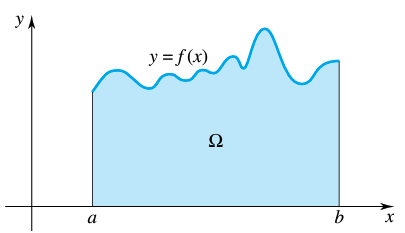
\includegraphics[width=.9\textwidth]{pics/area-bajo-curva.png}
\end{minipage}

\begin{example}
  Hallar el área debajo de la gráfica de la función raíz cuadrada entre $x=0$ y $x=1$.

  Como $\sqrt{x}\ge0$ para todo $x$, dicha área se calcula de la siguiente manera:
  \[
  \int_0^1 \sqrt{x}\dx = \int_0^1 x^{1/2}\dx 
  = \Big[ \frac{x^{1/2+1}}{1/2+1} \Big]_0^1
  = \Big[ \frac23x^{3/2} \Big]_0^1
  = \frac23 \cdot 1 - \frac23 \cdot 0 = \frac23.
  \]
\end{example}

\centerline{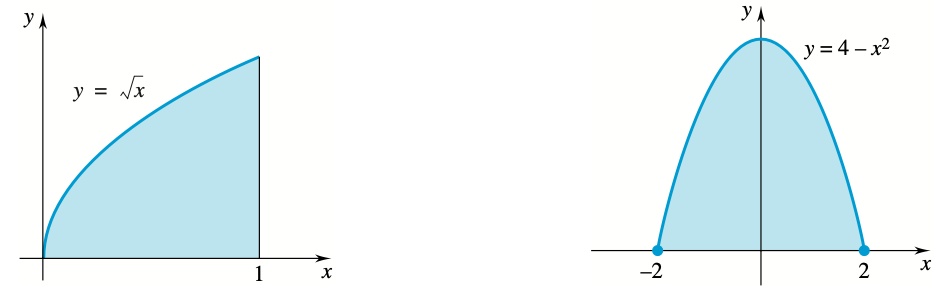
\includegraphics[width=.9\textwidth]{pics/areas-1.png}}

\begin{example}
  Hallar el área de la región comprendida entre la curva $y=4-x^2$ y el eje $x$.

  En este caso no nos dicen entre qué valores hay que tomar $x$. Entonces, tenemos que ver las intersecciones entre la curva $y=4-x^2$ y el eje $x$. Las intersecciones se encuentran en puntos con abscisas $x=-2$ y $x=2$ (ver figura).
  Luego calculamos el área integrando entre $-2$ y $2$:
  \[
  \int_{-2}^2 (4-x^2)\dx = \Big[ 4\, x-\frac13 x^3 \Big]_{-2}^2
  = \frac{32}3.
  \]
\end{example}

Consideremos ahora el área de la región $\Omega$ de la siguiente figura:

\centerline{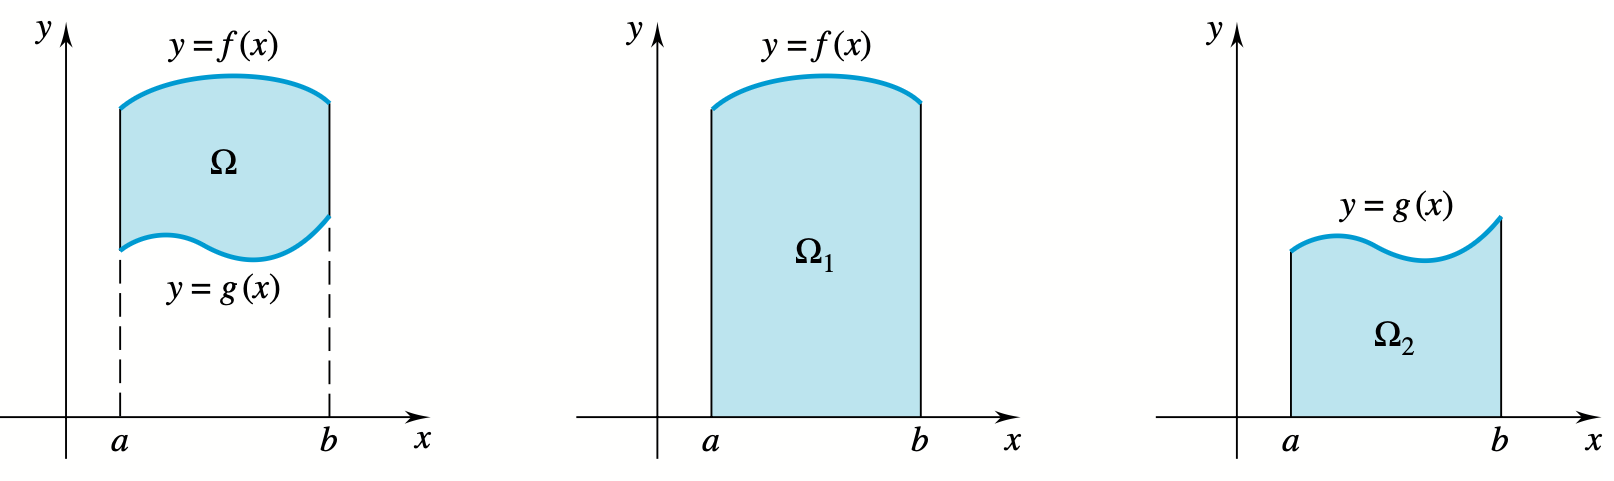
\includegraphics[width=.9\textwidth]{pics/areas-2.png}}

La frontera superior de $\Omega$ es la gráfica de la función no negativa $f$, y su frontera inferior es la gráfica de otra función no negativa $g$. Podemos obtener el área de $\Omega$ calculando el área de $\Omega_1$ y restándole el área de $\Omega_2$:
\begin{align*}
  \area(\Omega)&=\area(\Omega_1)-\area(\Omega_2)\\
  &= \int_a^b f(x)\dx - \int_a^b g(x)\dx.
\end{align*}
Por la linealidad de la integral, tenemos que
\begin{equation}\label{eq:area entre dos curvas}
  \area(\Omega) = \int_a^b \big[f(x)-g(x)\big]\dx.
\end{equation}

\begin{example}
  Hallemos el área de la región limitada por arriba por $y=x+2$ y por debajo por $y=x^2$.

  \noindent
  \begin{minipage}{.65\textwidth}
    El primer paso consiste en hallar los puntos de interseccipon de las dos curvas:
    \[
    x+2=x^2 \iff x^2-x-2=0 \iff x=-1 \text{ o } x=2.
    \]
    Por lo tanto las abscisas de los puntos de intersección son $x=-1$ y $x=-2$.
    Luego, el área de la región de interés es
    \begin{align*}
      \int_{-1}^2 \big[(x+2)-x^2\big]\dx 
      &= \Big[\frac{x^2}2+2x-\frac{x^3}3\Big]_{-1}^2
      \\ 
      &= \big[ 2 + 4 - \frac83\big]-\big[\frac12-2+\frac13\big]=\frac92.
    \end{align*}
  \end{minipage}
  \begin{minipage}{.34\textwidth}
    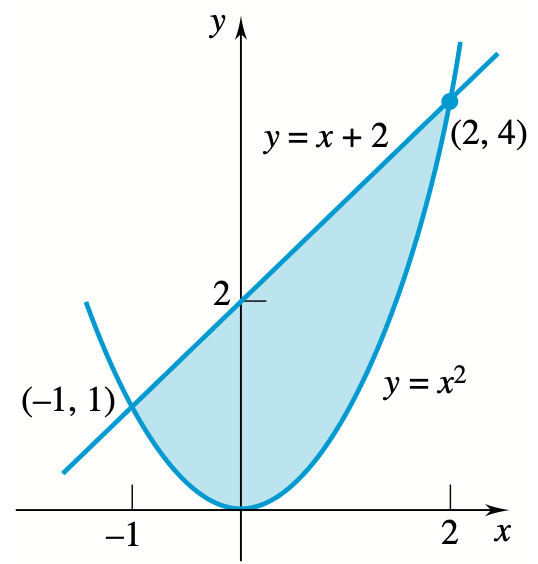
\includegraphics[width=.95\textwidth]{pics/areas-3.png}
  \end{minipage}
  \end{example}

  Hemos establecido la fórmula~\eqref{eq:area entre dos curvas} suponiendo que $f$ y $g$ son ambas no negarivas, pero esta hipótesis es innecesaria. La fórmula es válida para cualquier región $\Omega$ que tenga a $y=f(x)$ como frontera superior y a $y=g(x)$ como frontera inferior.
  Para ver esto, tomemos $\Omega$ como la figura de la izquierda y $\Omega'$ como la figura de la derecha:

  \begin{center}
    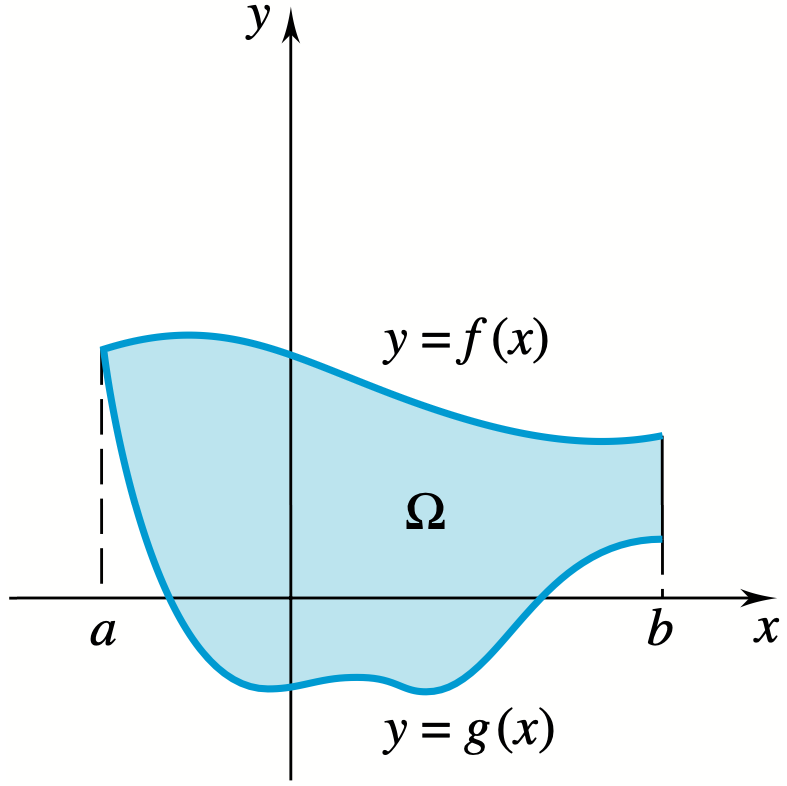
\includegraphics[width=.4\textwidth]{pics/areas-4a.png}
    \hfil
    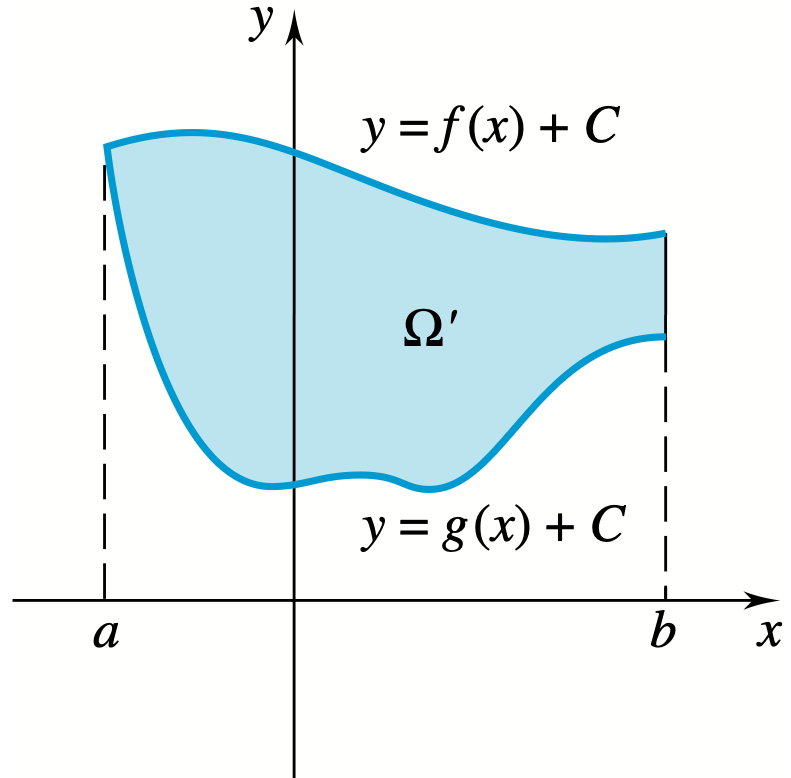
\includegraphics[width=.4\textwidth]{pics/areas-4b.png}
  \end{center}

  La figura $\Omega'$ es la misma que $\Omega$, pero trasladada hacia arriba $C$ unidades, y por lo tanto tienen la misma área. Entonces
  \[
  \area(\Omega)=\area(\Omega')
  =\int_a^b \Big[\big(f(x)+C\big)-\big(g(x)+C\big)\Big]\dx
  =\int_a^b \Big[f(x)-g(x)\Big]\dx.
  \]

  \begin{example}
    Consideramos ahora el problema de hallar el área de la figura de la derecha.

    \noindent
    \begin{minipage}{.55\textwidth}
      Usando la fórmula~\eqref{eq:area entre dos curvas} tenemos:
      \begin{align*}
        \area(\Omega) 
        &= \int_{\pi/4}^{5\pi/4} \big[\sen x-\cos x]\dx 
        \\
        &= \Big[-\cos x-\sen x\Big]_{\pi/4}^{5\pi/4}
        \\ 
        &= 2\sqrt{2}.
      \end{align*}
    \end{minipage}
    \begin{minipage}{.44\textwidth}
      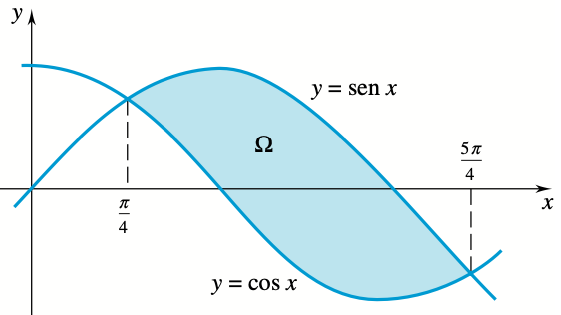
\includegraphics[width=.95\textwidth]{pics/areas-5.png}
    \end{minipage}    
  \end{example}

  \begin{example}
    Consideramos ahora el problema de hallar el área comprendida entre la curva $y=4x$ y la curva $y=x^3$, desde $x=-2$ hasta $x=2$.

    \noindent
    \begin{minipage}{.55\textwidth}
      Observamos que $y=x^3$ es la frontera \emph{superior} entre $x=-2$ y $x=0$, mientras que $y=x^3$ es la frontera \emph{inferior} entre $x=0$ y $x=2$.
      Luego,
      \begin{align*}
        \area
        &= 
        \int_{-2}^0 \big[x^3-4x\big]\dx 
        +
        \int_0^2 \big[4x-x^3\big]\dx 
        \\
        &= 
        \Big[\frac{x^4}4-2x^2\Big]_{-2}^0
        +
        \Big[4x-x^3\Big]_0^2 
        \\
        &= \big[0-(-4)\big]+[4-0]=8
      \end{align*}
    \end{minipage}
    \begin{minipage}{.44\textwidth}
      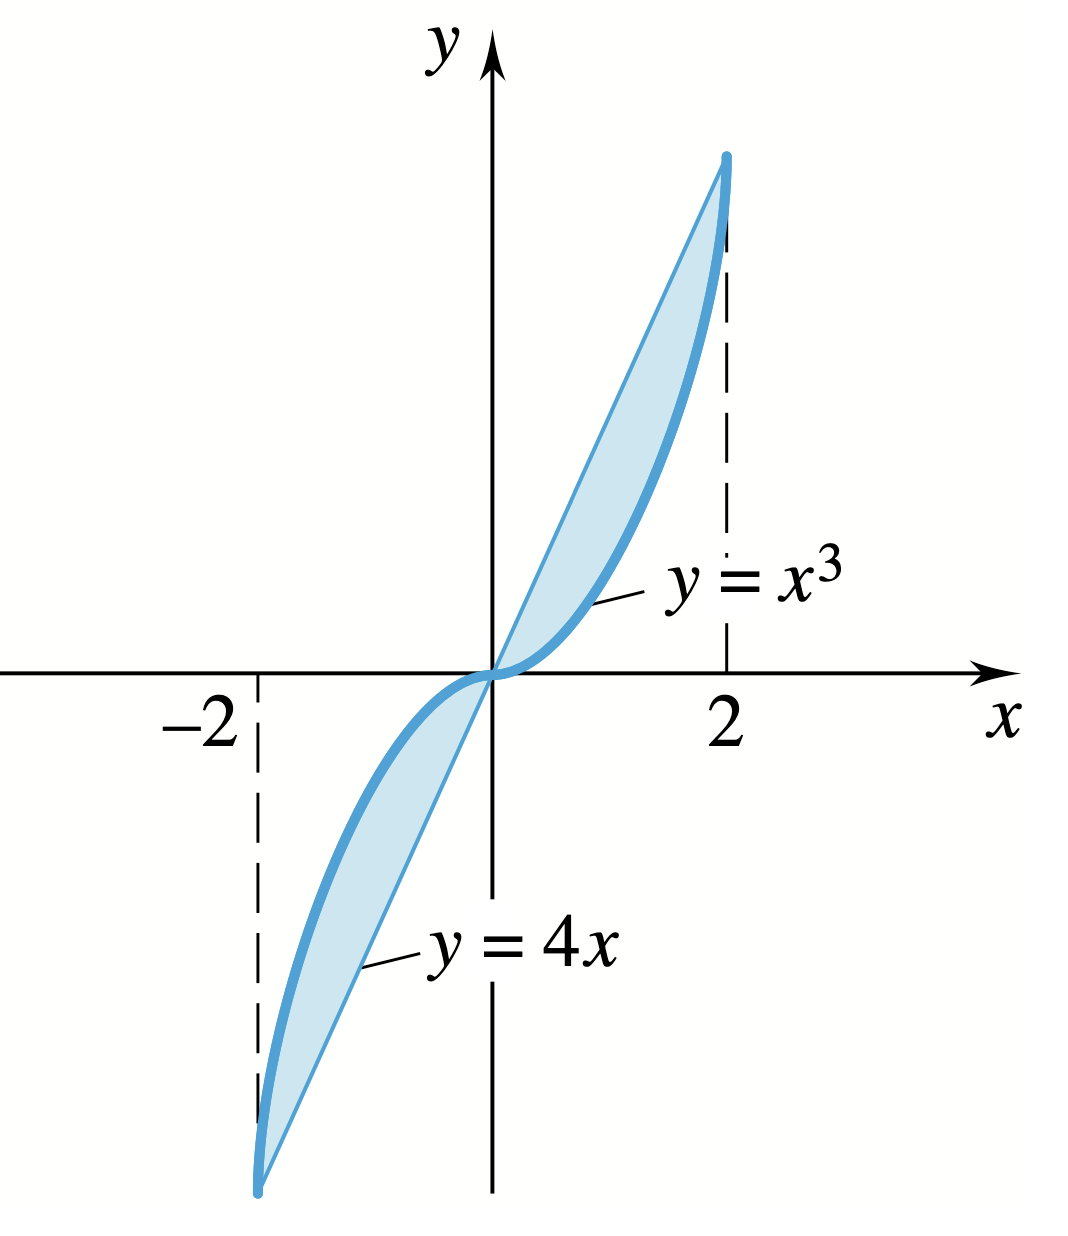
\includegraphics[width=.95\textwidth]{pics/areas-6.png}
    \end{minipage}    
  \end{example}

\subsubsection*{Ejercicios de la sección~\getcurrentref{chapter}.\getcurrentref{section}}

\begin{enumerate}
  \item Dibujar la región limitada por las curvas y calcular su área.
\begin{multicols}{2}
  \begin{enumerate}
    \item $\D y= \sqrt x$,\quad $\D y= x^2$.
    \item $\D y= 8-x^2$,\quad $\D y= x^2 $.
    \item $\D y= 5-x^2$,\quad $\D y= 3-x $.
    \item $\D y^2=2x$,\quad $\D x-y=4  $.
    \item $\D x-y^2+3=0 $,\quad $\D x-2y=0  $.
  \end{enumerate}
  
\end{multicols}
\end{enumerate}  


\section{Integrales indefinidas}

Consideremos una función continua $f$. Si $F$ es una antiderivada de $f$ en $[a,b]$, entonces
\[
\int_a^b f(x)\dx = \Big[F(x)\Big]_a^b = F(b)-F(a).
\]
Si $C$ es una constante, 
\[
  \Big[F(x)+C\Big]_a^b 
  = \big[F(b)+C\big]-\big[F(a)+C\big]= F(b)-F(a)
  = \Big[F(x)\Big]_a^b = \int_a^b f(x)\dx.
\]
Esto es así porque $F(x)+C$ es también una antiderivada de $f$ ya que
\[
\dd[]{}{x} \big(F(x)+C\big) = F'(x) = f(x).
\]
Y además, \emph{todas} las antiderivadas de $f$ son de la forma $F(x)+C$, con $C$ una constante.

Si no tenemos un interés especial en el intervalo $[a,b]$ y sólo queremos resaltar el hecho que $F$ es una antiderivada de $f$ para algún intervalo, entonces omitiremos $a$ y $b$ y simplemente escribiremos
\[
\int f(x)\dx = F(x)+C.
\]
Cuando se expresan de este modo, las antiderivadas se llaman \emph{integrales indefinidas}.
La consstante $C$ se denomina \emph{constante de integración}; es una constante \emph{arbitraria} porque se le puede asignar cualquier valor real.

La integral indefinida de una función $f$, es $\int f(x)\dx$, y es una \emph{familia} de funciones: es la familia de \emph{todas} las antiderivadas de $f$. Por ejemplo:
\[
\int x^2\dx = \frac{x^3}{3} + C 
\qquad\text y \qquad
\int \sqrt{s}\ds = \frac23 s^{3/2}+C.
\]
En base a la tabla de derivadas y a los ejercicios del capítulo anterior tenemos la siguiente tabla de integrales indefinidas:

\begin{multicols}{2}
  $\D \int x^\alpha \dx = \frac{x^{\alpha+1}}{\alpha+1} + C$, si $\alpha\neq -1$
  
  $\D \int \frac1x\dx = \ln|x| + C$
  
  $\D \int a^x \dx = \ln a\cdot a^x  + C$, si $a>0$
  
  $\D \int \sen x\dx = -\cos x + C$
  
  $\D \int \cos x \dx = \sen x + C$
  
  $\D \int \sec^2 x\dx = \tan x + C$
  
  $\D \int \cosec^2 x\dx = \cot x + C$
  
  $\D \int \senh x \dx = \cosh x + C$
  
  $\D \int \cosh x \dx = \senh x + C$
  
\end{multicols}

Las propiedades de linealidad de la integral definida son también válidas para la integral indefinida:
\[
\int c\, f(x)+g(x)\dx = c \int f(x)\dx + \int g(x)\dx.
\]
Así, por ejemplo
\[
\int 3x^5 + 6 \sen x \dx = \frac{x^6}2 - 6 \cos x + C.
\]

\begin{example}
  Hallar $f$ sabiendo que $\D f'(x)=x^3+2$ y $f(0)=1$.

  Dado que $f'$ es la derivada de $f$, $f$ es una antiderivada de $f'$. Luego
  \[
  f(x)=\int (x^3+2)\dx = \frac{x^4}{4}+2x+C ,
  \]
  para algún valor de la constante $C$.
  Para hallar $C$ usaremos el hecho que $f(0)=1$:
  \[
  1=f(0)=\frac{0^4}{4}+2\cdot 0+C = C, 
  \]
  y obtenemos que $C=1$. Luego
  $\D f(x)= \frac{x^4}{4}+2x+1$.
\end{example}

\begin{example}\label{ej:velocidad}
  Consideremos un problema de movimiento.
  Un objeto se mueve a lo largo de un eje de coordenadas con una velocidad de 
  \[
  v(t)=2-3t+t^2\text{\ \ unidades por segundo.}
  \]
  Su posición inicial (posición en el instante $t=0$) es de 2 unidades a la derecha del origen.
  Hallar la posición del objeto 4 segundos más tarde.

  Sea $s(t)$ la (coordenada de la) posición del objeto en el instante $t$.
  Sabemos que $s(0)=2$ y que $s'(t)=v(t)$, luego
  \[
  s(t)=\int v(t)\dt = \int (2-3t+t^2 )\dt = 2t -\frac32 t^2 +\frac{t^3}3 + C.
  \]
  Para conocer la constante $C$ utilizaremos que $s(0)=2$:
  \[
  2=s(0)=2\cdot 0 -\frac32 0^2 +\frac{0^3}3 + C = C.
  \]
  Luego $C=2$ y la posición del objeto a tiempo $t$ es $\D 2t -\frac32 t^2 +\frac{t^3}3 +2$. A tiempo $t=4$ es 
  \[
  s(4)=2\cdot 4 -\frac32 4^2 +\frac{4^3}3 +2=\frac{22}3.
  \]
  Pasados 4 segundos se encuentra a $\D\frac{22}3$ unidades a la derecha del origen.
  En la figura se reresenta esquemáticamente el movimiento del objeto.

  \begin{center}
    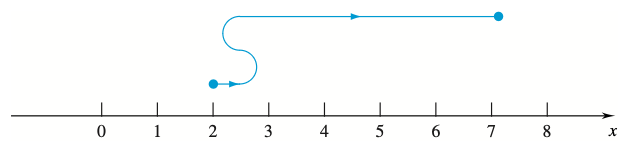
\includegraphics[width=.7\textwidth]{pics/movimiento.png}
  \end{center}

\end{example}

\subsubsection*{Ejercicios de la sección~\getcurrentref{chapter}.\getcurrentref{section}}

\begin{enumerate}
  \item Calcular las siguientes integrales indefinidas:
\begin{multicols}{2}
  \begin{enumerate}
    \item $\D \int \frac{1}{x^4} \dx$
    \item $\D \int \big(ax+b\big) \dx$
    \item $\D \int \frac{1}{\sqrt{1+x}} \dx$
    \item $\D \int \bigg(\frac{x^3-1}{x^2}\bigg) \dx$
    \item $\D \int \bigg(\sqrt{x}-\frac{1}{\sqrt{x}}\bigg) \dx$
    \item $\D \int \big(\sen x+\cos x\big) \dx$
    \item $\D \int \big(\senh x+\cosh x\big) \dx$
    \item $\D \int \frac{g'(x)}{g(x)^2} \dx$
  \end{enumerate}
\end{multicols}

\item Hallar $f$ a partir de la información dada:
\begin{multicols}{2}
  \begin{enumerate}
    \item $f'(x)=2x-1$,\ \ $f(3)= 0$
    \item $f'(x)=ax+b$,\ \ $f(0)=c $
    \item $f'(x)=\sen x$,\ \ $f(0)= 2$
    \item $f'(x)=\cos x$,\ \ $f(\pi )=3 $
  \end{enumerate}
\end{multicols}

\item Un objeto se mueve a lo largo de un eje de coordenadas con una velocidad de $v(t)=6t^2-6$ metros por segundo. Su posición inicial (posición en tiempo $t=0$) es 2 unidades a la izquierda del origen.
\begin{enumerate}
  \item Hallar la posición del objeto $3$ segundos más tarde.
  \item Representar esquemáticamente el movimiento del objeto como en el Ejemplo~\ref{ej:velocidad}.
  \item ?`Cuál es la distancia entre la posición del objeto a tiempo $t=0$ y la posición a tiempo $t=3$?
  \item ?`Cuál es la distancia total recorrida por el objeto entre tiempo $t=0$ y $t=1$?
\end{enumerate}
\end{enumerate}    


\section{Integración por sustitución}

La integración por sustitución, también conocida como \emph{cambio de variables} no es otra cosa que la utilización de la regla de la cadena en sentido inverso para hallar una antiderivada.
Recordamos que si $F$ y $g$ son diferenciables, con $F'(u)=f(u)$, entonces
\[
(F\circ g)'(x) = \dd[]{}{x} F\big(g(x)) = F'(g(x))\, g'(x) = f(g(x))\, g'(x).
\]
Por lo tanto, 
\[
\int_a^b f(g(x))\, g'(x)\dx = \Big[F(g(x))\Big]_a^b = F(g(b))-F(g(a)).
\]

Por ejemplo:
\[
\int_0^\pi \cos(x^2+1)\, 2x \dx = \Big[\sen(x^2+1)\Big]_0^\pi = 
\sen(\pi^2+1)-\sen(0^2+1).
\]
En el ejemplo recién presentado hemos detectado que $\cos(u)$ es la derivada de $\sen(u)$, y que $2x$ es la derivada de $u=x^2+1$.

También podemos usar la regla de sustitución para calcular una integral indefinida. Esto es lo más usual, y suele hacerse de la siguiente manera:
\[
\int f(\underbrace{g(x)}_u) \, \underbrace{g'(x)\dx}_{\du} = 
\int f(u) \du = F(u)+C = F(g(x))+C.
\]
Por ejemplo, 
\[
\int (\underbrace{x^2-1}_u)^4\, \underbrace{2x\dx}_{\du} = \int u^4 \du 
= \frac{u^5}5 + C
= \frac{(x^2-1)^5}5 + C.
\]
Podemos verificar esto derivando la última expresión:
\[
\dd[]{}{x} \left(\frac{(x^2-1)^5}5 + C\right) =
\frac{5(x^2-1)^4\,2x}5 = (x^2-1)^4\, 2x.
\]

\begin{example}
  Calcular $\D \int \sen x\,\cos x\dx$.

  El problema aquí es \emph{darse cuenta} qué parte de la fórmula puede ser $u$ y qué parte será $\du$. 
  Si recordamos que $\sen'x = \cos x$, vemos que podemos hacer la sustitución $u=\sen x$ y $\du = \cos x\dx$, entonces
  \[
  \int \underbrace{\sen x}_u\,\underbrace{\cos x\dx}_{\du} = \int u \du = \frac{u^2}2 + C 
  \underbrace{=}_{u=\sen x} \frac{\sen^2 x}{2}+ C.
  \]
  Conviene siempre hacer la verificación:
  \[
  \dd[]{}{x}\Big(\frac{\sen^2 x}{2}+ C\Big) = \frac{2 \sen x \, \cos x}2 = \sen x\,\cos x.
  \]
\end{example}

\begin{example}
  Calcular $\D \int \frac{1}{(3+5x)^2}\dx$. 
  
  Aquí no es tan obvio que aparezca $u$ y $\du$, pero con un poco de práctica se aprende.
  Si tomamos $u=(3+5x)$, entonces $\du = 5\dx$, pero ese $5$ no está. Usando la linealidad de la integral, como $5$ es una constante, podemos hacer lo siguiente:
  \begin{align*}
    \int \frac{1}{(3+5x)^2}\dx &= \int \frac55 \frac{1}{(3+5x)^2}\dx
    = \frac15 \int \frac{1}{(\underbrace{3+5x}_u)^2} \underbrace{5\dx}_{\du}
    = \frac15 \int \frac{1}{u^2} \du 
    \\
    &= \frac15 \int u^{-2} \du
    = \frac15 \Big(\frac{u^{-1}}{-1}+C\Big)
    = \frac15 \Big(-\frac{1}{u}+C\Big)
    \\
    &= -\frac{1}{5u}+\frac{C}5
    = -\frac{1}{5u}+C'
    = -\frac{1}{5(3+5x)^2}+C'.
  \end{align*}
\end{example}

Si tenemos que calcular una integral definida utilizando el método de sustitución, hay dos formas (por lo menos).
La primera es la siguiente: calcular primero la integral indefinida (basta con una antiderivada) y luego utilizarla para integrar.

\begin{example}
  Calcular $\D \int_0^2 (x^2-1) \, (x^3-3x+2)^3 \dx$.

  Hacemos aquí la sustitución $u=x^3-3x+2$ y $\du = 3x^2-3\dx=3(x^2-1)\dx$,
  y miramos la integral indefinida:
  \begin{align*}
    \int (x^2-1) \, (x^3-3x+2)^3 \dx &= \frac13 \int  (x^3-3x+2)^3\, 3(x^2-1) \dx
    \\
    &=\frac13\int u^3 \du = \frac{u^4}{12} + C = \frac{(x^3-3x+2)^4}{12} + C.
  \end{align*}
  Es decir, hemos encontrado que $\frac{(x^3-3x+2)^4}{12}$ es una antiderivada del integrando.
  Luego
  \begin{align*}
    \int_0^2 (x^2-1) \, (x^3-3x+2)^3 \dx 
    &= \Big[
      \frac{(x^3-3x+2)^4}{12}
      \Big]_0^2
      \\
      &= \frac{(2^3-3\cdot 2+2)^4}{12} - \frac{(0^3-3\cdot 0+2)^4}{12}
      \\
      &=   \frac{(8-6+2)^4}{12} - \frac{2^4}{12} = 20.
  \end{align*}  
\end{example}

La segunda forma será vista luego del siguiente teorema:

\begin{theorem} 
  Si $f$ es continua y $g$ es tal que $g'$ es continua, entonces
  \[
  \int_a^b f(g(x))\, g'(x)\dx = \int_{g(a)}^{g(b)} f(u)\du.
  \]
\end{theorem}

\begin{proof}
  Sea $F$ una antiderivada de $f$. Entonces $F'(u)=f(u)$ y 
  \begin{align*}
    \int_a^b f(g(x))\, g'(x)\dx 
    &= \int_a^b F'(g(x))\, g'(x)\dx \\
    &= \Big[ F(g(x))\Big]_a^b = F(g(b))-F(g(a)) 
    \\
    &= \Big[ F(u)\Big]_{g(a)}^{g(b)} = \int_{g(a)}^{g(b)} f(u) \du. 
    \qedhere
  \end{align*}
\end{proof}

Lo importante a notar en esta fórmula, es que si aplicamos la regla de sustitución en una integral \emph{definida}, también hay que sustituir en los extremos de integración.

\begin{example}
  Calcular $\D\int_0^{1/2} \cos^3 \pi x\,\sen\pi x\dx$.
  Hacemos la sustitución $u=\cos\pi x$ y $\du = -\pi \sen\pi x \dx$:
  \begin{align*}
    \int_0^{1/2} \cos^3 \pi x\,\sen\pi x\dx 
    &= -\frac1\pi \int_0^{1/2} \cos^3 \pi x\,(-\pi\,\sen\pi x)\dx \\
    &= -\frac1\pi \int_{\cos \pi 0}^{\cos \pi 1/2} u^3 \du 
    = -\frac1\pi \int_{1}^{0} u^3 \du \\
    &= -\frac1\pi  \Big[\frac{u^4}{4}\Big]_{1}^{0} 
    = -\frac1\pi  \Big[\frac{0^4}{4}-\frac{1^4}{4}\Big]_{1}^{0} 
    = -\frac1\pi  \Big[0-\frac{1}{4}\Big]
    = \frac{1}{4\pi}.
  \end{align*}
\end{example}

Para finalizar la sección, veamos un último ejemplo de sustitución en una integral indefinida 

\begin{example}
  Calcular $\D\int 2x \sqrt{x-1}\dx$.

  Aquí tenemos $x$ fuera de la raíz y $x-1$ dentro de la raíz. Parece que no podríamos hacer nada. Sin embargo, si hacemos la sustitución $u=x-1$ (nos queda $x=u+1$) y $\du = \dx$:
  \begin{align*}
    \int 2\underbrace{x}_{u+1} \sqrt{\underbrace{x-1}_u}\underbrace{\dx}_{\du}
    &= \int 2 (u+1)\sqrt{u}\du = 2 \int u^{3/2}+u^{1/2}\du
    \\
    &= 2\Big[ \frac{u^{5/2}}{5/2} + \frac{u^{3/2}}{3/2}\Big]
    = \frac45 u^{5/2} + \frac43 u^{3/2}
    =  \frac45 (x-1)^{5/2} + \frac43 (x-1)^{3/2}.
  \end{align*}
\end{example}

\subsubsection*{Ejercicios de la sección~\getcurrentref{chapter}.\getcurrentref{section}}

\begin{enumerate}
  \item Calcular las siguientes integrales indefinidas mediante el método de sustitución:

\begin{multicols}{2}
  \begin{enumerate}
    \item $\D \int \frac{1}{(2-3x)^2} \dx$.
    \item $\D \int \sqrt{ax+b} \dr$.
    \item $\D \int \frac{t}{(4t^2+9)^2} \dt$.
    \item $\D \int x^2 (1+x^3)^{1/4} \dx$.
    \item $\D \int \frac{b^3 \, x^3}{\sqrt{1-a^4x^4}} \dx$.
    \item $\D \int \frac{1}{4x+6}\dx$.
    \item $\D \int \frac{x^3}{1+x^4}\dx$.
    \item $\D \int e^{ax+b}\dx$.
    \item $\D \int x^3 e^{x^4+1}\dx$.
  \end{enumerate}
\end{multicols}

\item Calcular las siguientes integrales definidas mediante el método de sustitución:

\begin{multicols}{2}
  \begin{enumerate}
    \item $\D \int_{0}^{1} x(x^2+1)^3 \dx$.
    \item $\D \int_{-1}^{1} \frac{r}{(1+r^2)^4} \dr$.
    \item $\D \int_{0}^{3} \frac{r}{\sqrt{r^2+16}}  \dr$.
    \item $\D \int_{0}^{a} y\sqrt{a^2-y^2} \dy$.
  \end{enumerate}
\end{multicols}

\item Calcular las siguientes integrales indefinidas utilizando el cambio de variables indicado:

\begin{multicols}{2}
  \begin{enumerate}
    \item $\D \int x \sqrt{x+1} \dx $, $u = x+1$.
    \item $\D \int x \sqrt{2x-1} \dx $, $u = 2x-1$.
    \item $\D \int t\,(2t+3)^8 \dt $, $u = 2t+3$.
    \item $\D \int \frac{x+3}{\sqrt{x+1}}\dx $, $u = x+1$.
  \end{enumerate}
\end{multicols}
\end{enumerate}  

\section{Integración por partes}
% sección 9.3 de Noriega

En la sección anterior hemos visto cómo la regla de la cadena para la derivada de una composición nos permite calcular derivadas de funciones más complejas.
También hay una regla de integración asociada con la regla de la derivada de un producto.

Sean $u$ y $v$ dos funciones derivables. Por la Proposición~\ref{P:derivada del producto} tenemos que
\[
(uv)'=u'v + u v',
\]
o sea 
\[
  u'v =(uv)'- u v'.
\]
Entonces resulta que 
$$
\int u'v \dx = \int (uv)' \dx - \int u v'\dx.
$$

Tenemos entonces el siguiente Teorema.

\begin{theorem}[Integración por partes]
  Si $u$ y $v$ son funciones diferenciables tales que $u'$ y $v'$ son continuas, entonces 
  \[
  \int_a^b u'(x)v(x) \dx = \Big[u(x)v(x)\Big]_a^b - \int_a^b u(x) v'(x)\dx,
  \]
  es decir,
  \[
  \int_a^b u'(x)v(x) \dx 
  = u(b)v(b)-u(a)v(a) - \int_a^b u(x) v'(x)\dx.
  \]
\end{theorem}

\begin{proof}
  Por la regla de la derivada del producto, Proposición~\ref{P:derivada del producto} tenemos que $(uv)'(x)=u'(x)v(x) + u(x) v'(x)$. Luego, $(uv)(x)=u(x)v(x)$ es una antiderivada de $u'(x)v(x) + u(x) v'(x)$. Por la linealidad de la integral y por la regla de Barrow tenemos que
  \begin{align*}
  \int_a^b u'(x)v(x) \dx+ \int_a^b u(x) v'(x) \dx
  &=\int_a^b u'(x)v(x) + u(x) v'(x) \dx
  \\
  &= \int_a^b (uv)'(x)\dx 
  = \Big[(uv)(x)\Big]_a^b  
  \\
  &= \Big[u(x)v(x)\Big]_a^b  
  = u(b)v(b)-u(a)v(a),
  \end{align*}
  de donde se deduce inmediatamente la afirmación del teorema.
\end{proof}

Otra forma de escribir la \emph{fórmula de integración por partes} es la siguiente:
$$
\int u'v \dx = uv - \int u v'\dx.
$$

Veamos cómo se puede aplicar esta regla en ejemplos concretos.

\begin{example}
  Calcular $\D\int x\,\ln x\dx$.

  Aquí hacemos $u=\ln x$ y $v'=x$. Luego $\D u'=\frac1x$ y $\D v=\frac{x^2}2$. Luego
  \[
  \int x \ln x\dx 
  = \ln x \, \frac{x^2}2 - \int \frac1x \frac{x^2}{2}\dx
  = \ln x \, \frac{x^2}2 - \int \frac{x}{2}\dx
  = \ln x \, \frac{x^2}2 - \frac{x^2}{4} + C.
  \]  
\end{example}

\begin{example}
  Calcular $\D \int x e^x\dx$.

  En este ejemplo, la idea es aprovechar que $\dd[]{x}{x}=1$ y que $\dd[]{e^x}{x}=e^x$. Entonces tomamos $u=x$, y $v'=e^x$. Luego, $u'=1$ y $v=e^x$:
  \[
  \int x\, e^x\dx = x\,e^x - \int 1 e^x\dx = x\, e^x - e^x+C = (x-1)e^x+C.
  \]
\end{example}

\begin{example}
  Calcular $\D \int x^2 e^x\dx$.

  En este ejemplo, la idea es repetir dos veces la fórmula para poder \emph{deshacernos} de la potencia de $x$. Tomamos primero $u=x^2$, y $v'=e^x$. Luego, $u'=2x$ y $v=e^x$:
  \[
  \int x^2\, e^x\dx 
  = x^2\,e^x - \int 2x e^x\dx 
  = x^2\,e^x - 2\int x e^x\dx .
  \]
  Llegado a este punto nos tocaría aplicar nuevamente la integración por partes en el último término, pero como lo hemos hecho en el ejemplo anterior, podemos copiar la fórmula de allí.
  \[
  \int x^2\, e^x\dx 
  = x^2\,e^x - 2\int x e^x\dx 
  = x^2\,e^x - 2(x\, e^x - e^x) + C
  = (x^2-2x+2)\,e^x + C.
  \]
\end{example}

Veamos un último ejemplo.

\begin{example}
  Calcular $\D \int e^x\, \cos x \dx$.

  Aquí integraremos por partes dos veces. Primero escribimos
  $u=e^x$ y $v'=\cos x$, con $u'=e^x$ y $v=\sen x$. Esto nos da
  \[
  \int e^x\,\cos x \dx 
  = e^x \,\sen x - \int e^x \,\sen x\dx .
  \]
  Ahora hacemos integración por partes en $\D \int e^x \, \sen x \dx$.
  En este caso, tomamos $u=e^x$ y $v'=\sen x$, con $u'=e^x$ y $v=-\cos x$. Luego
  \[
  \int e^x\,\sen x \dx 
  = e^x (-\cos x) - \int e^x (-\cos x)\dx 
  = -e^x \,\cos x + \int e^x \, \cos x \dx .
  \]
  Juntando todo,
  \begin{align*}
    \int e^x\,\cos x \dx 
    &= e^x \,\sen x -\Big[-e^x \,\cos x + \int e^x \, \cos x \dx \Big]\\
    &= e^x \,\sen x +e^x \,\cos x - \int e^x \, \cos x \dx .
  \end{align*}
  Es decir
  \[
    \int e^x\,\cos x \dx 
    = e^x\big(\sen x+\cos x) - 
    \int e^x\,\cos x \dx .
  \]
  Por lo tanto 
  \[
    2\int e^x\,\cos x \dx 
    = e^x\big(\sen x+\cos x),
  \]
  y finalmente 
  \[
    \int e^x\,\cos x \dx 
    = \frac{e^x}2\big(\sen x+\cos x) + C.
  \]
\end{example}



\subsubsection*{Ejercicios de la sección~\getcurrentref{chapter}.\getcurrentref{section}}

\begin{enumerate}
  \item Calcular las siguientes integrales:
\begin{multicols}{2}
  \begin{enumerate}
    \item $\D \int x\,e^{-x} \dx$.
    \item $\D \int_0^2 x \, 2^x  \dx$.
    \item $\D \int x^2\, e^{-x^3} \dx$.
    \item $\D \int x \, \ln x^2 \dx$.
    \item $\D \int_0^1 x^2\, e^{-x} \dx$.
    \item $\D \int \frac1{x\, (\ln x)^3} \dx$.
    % \item $\D \int  \dx$.
  \end{enumerate}
  
\end{multicols}
\item Hallar el área de la región limitada por la gráfica de $f$ y el eje $x$:
\begin{multicols}{2}
  \begin{enumerate}
    \item $f(x)=\arcsen x$, $x\in[0,1/2]$.
    \item $f(x)=x\,e^{-2x}$,  $x\in[0,2]$.
  \end{enumerate}
\end{multicols}
\end{enumerate}  


\section{Algunas propiedades adicionales de la integral}

En esta sección veremos algunas propiedades generales importantes de la integral definida. En todos los resultados presentados en esta sección estamos suponiendo que $a<b$.

\begin{lemma}\label{L:integral ge 0}
  Si $f$ es continua a trozos y $f(x)\ge 0$, para todo $x\in [a,b]$, entonces 
  \[
  \int_a^b f(x)\dx \ge 0.
  \]
\end{lemma}

\begin{proof}
  Hacemos la demostración para el caso en que $f$ es continua.
  Como $f$ es continua en $[a,b]$, alcanza su mínimo, digamos en un punto $x_m$, donde $f(x_m)\ge 0$ por hipótesis. Tomemos ahora la partición $P=\{x_0=a<x_1=b\}$.
  Luego 
  \[
  L(P,f)=f(x_m) (b-a)=\ell \ge 0.
  \]
  Por lo tanto la integral, que es un número mayor o igual a todas las sumas inferiores tiene que ser también mayor o igual que $\ell\ge0$ y por lo tanto es no negativa.
\end{proof}

\begin{lemma}\label{L:integral > 0}
  Si $f$ es continua a trozos y $f(x)> 0$, para todo $x\in [a,b]$, entonces
  \[
  \int_a^b f(x)\dx > 0.
  \]
\end{lemma}

\begin{proof}
  Hacemos la demostración para el caso en que $f$ es continua.
  Como $f$ es continua en $[a,b]$, alcanza su mínimo, digamos en un punto $x_m$, donde $f(x_m)>0$ por hipótesis. Tomemos ahora la partición $P=\{x_0=a<x_1=b\}$.
  Luego 
  \[
  L(P,f)=f(x_m) (b-a)=\ell > 0.
  \]
  Por lo tanto la integral, que es un número mayor o igual a todas las sumas inferiores tiene que ser también mayor o igual que $\ell>0$ y por lo tanto es positiva.
\end{proof}

\begin{proposition}
  Si $f$ y $g$ son continuas a trozos y $f(x)\le g(x)$ para todo $x\in[a,b]$, entonces
  \[
  \int_a^b f(x)\dx 
  \le \int_a^b g(x)\dx 
  \]
\end{proposition}

\begin{proof}
  Aplicar el Lema~\ref{L:integral ge 0} a la función $h(x)=g(x)-f(x)$.
\end{proof}

\begin{proposition}\ref{P:integral monotona}
  Si $f$ y $g$ son continuas a trozos y $f(x) < g(x)$ para todo $x\in[a,b]$, entonces
  \[
  \int_a^b f(x)\dx 
  \le \int_a^b g(x)\dx 
  \]
\end{proposition}

\begin{proof}
  Aplicar el Lema~\ref{L:integral > 0} a la función $h(x)=g(x)-f(x)$.
\end{proof}

De la misma manera que el valor absoluto de una suma es menor o igual que la suma de los valores absolutos:
\[
|f_1+f_2+\dots+f_n| \le |f_1|+|f_2|+\dots+|f_n| ,
\]
el valor absoluto de una integral es menor o igual que la integral del valor absoluto.

\begin{corollary}
  Si $f$ es continua a trozos en $[a,b]$ entonces
  \[
  \Big| \int_a^b f(x)\dx \Big| \le \int_a^b |f(x)|\dx.
  \]
\end{corollary}

\begin{proof}
  Dado que $\D -|f(x)|\le f(x)\le |f(x)|$, la Proposición~\ref{L:integral monotona} nos dice que
  \[
    -\int_a^b |f(x)|\dx 
    \le \int_a^b f(x)\dx 
    \le \int_a^b |f(x)|\dx .
  \]
  Este par de desigualdades equivale a la afirmación que queremos demostrar.
\end{proof}

\subsubsection*{Ejercicios de la sección~\getcurrentref{chapter}.\getcurrentref{section}}

\begin{enumerate}
  \item Supongamos que $f$ y $g$ son continuas, $a<b$ y 
\[
\int_a^b f(x)\dx > \int_a^b g(x)\dx.
\]
\begin{enumerate}
  \item ?`Se deduce necesariamente que $\int_a^b \big[ f(x)-g(x)\big]\dx > 0$?
  \item ?`Se deduce necesariamente que $f(x)>g(x)$, para todo $x\in [a,b]$?
  \item ?`Se deduce necesariamente que existe $x\in[a,b]$ tal que $f(x)>g(x)$?
  \item ?`Se deduce necesariamente que $\Big|\int_a^b f(x)\dx\Big| > \Big|\int_a^b g(x)\dx\Big| $?
\end{enumerate}

\item Supongamos que $f$ es continua, $a<b$ y 
\[
\int_a^b f(x)\dx =0.
\]
\begin{enumerate}
  \item ?`Se deduce necesariamente que $f(x)=0$, para todo $x\in [a,b]$?
  \item ?`Se deduce necesariamente que existe $x\in[a,b]$ tal que $f(x)=0$?
  \item ?`Se deduce necesariamente que $\Big|\int_a^b f(x)\dx\Big| =0 $?
  \item ?`Se deduce necesariamente que $\int_a^b |f(x)|\dx =0 $?
\end{enumerate}
\end{enumerate}



\section{Integrales impropias}



\subsubsection*{Ejercicios de la sección~\getcurrentref{chapter}.\getcurrentref{section}}

\begin{enumerate}
  \item La base de un sólido es el círculo $x^2 + y^2 = 7$. Hallar el volumen de dicho sólido si las secciones transversales perpendiculares al eje $x$ son
\begin{multicols}{2}
  \begin{enumerate}
    \item Cuadrados.
    \item Triángulos equiláteros.
  \end{enumerate}
\end{multicols} 

\item La base de un sólido es la región limitada por la elipse $4x^2 + 9y^2 = 36$. Hallar el volumen del sólido sabiendo que las secciones transversales perpendiculares al eje $x$ son
\begin{multicols}{2}
  \begin{enumerate}
    \item Triángulos equiláteros.
    \item Cuadrados.
  \end{enumerate}
\end{multicols} 

\item La base de un sólido es la región limitada por $y = x^2$ e $y = 4$. Hallar el volumen sabiendo que las secciones perpendiculares al eje $x$ son:
\begin{multicols}{2}
  \begin{enumerate}
    \item Cuadrados.
    \item Semicírculos.
    \item Triángulos equiláteros.
  \end{enumerate}
\end{multicols} 

\item La base de un sólido es la región comprendida entre las parábolas $x = y^2$ y $x = 3 - 2y^2$. Hallar el volumen del sólido sabiendo que las secciones perpendiculares al eje $x$ son 
\begin{multicols}{2}
  \begin{enumerate}
    \item Rectángulos de altura $h$.
    \item Triángulos equiláteros.
    \item Triángulos rectángulos isósceles, cada uno con la hipotenusa sobre el plano $xy$
  \end{enumerate}
\end{multicols} 

\item Hallar la fórmula para el volumen de un cono truncado en
función de su altura $h$, el radio de la base inferior $R$ y el radio de
la base superior $r$.

\centerline{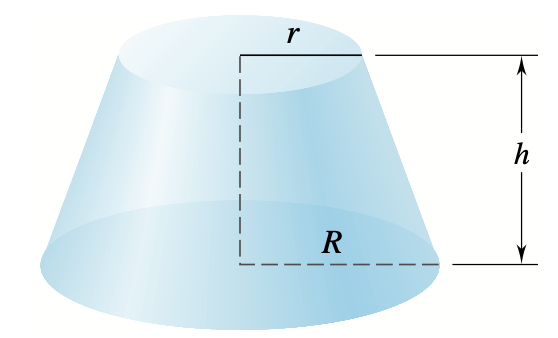
\includegraphics[width=.3\textwidth]{pics/cono-truncado.png}}

\item Un plano corta una esfera de radio $r$ a una altura de $h$ unidades
por encima del ecuador ($0 < h < r$). La parte superior de la
esfera se llama casquete. Deducir la fórmula de su volumen.

\item  La región que se muestra en la figura se rota alrededor de eje $y$
para formar un recipiente de forma parabólica. La unidades
indicadas están en metros. ?`Cuál es el volumen del recipiente?

\centerline{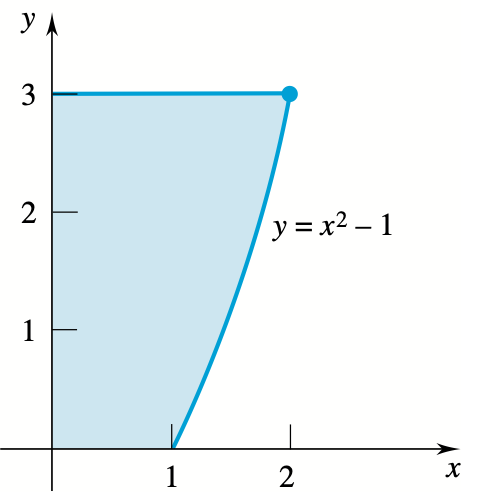
\includegraphics[width=.3\textwidth]{pics/recipiente-parabolico.png}}


\end{enumerate}


\section{El método de integración por fracciones simples}


\subsubsection*{Ejercicios de la sección~\getcurrentref{chapter}.\getcurrentref{section}}

\begin{enumerate}
\item 
\end{enumerate}



\subsection*{Ejercicios del capítulo~\getcurrentref{chapter}}



